%%%%%%%%%%%%%%%%%%%%%%%%%%%%%%%%%%%%%%%%%%%%%%%%%%%%%%%%%%%%%%%%%%%%%%
%% Risk-Optimal Momentum Weights for Stochastic Gradient Estimation  %%
%% in High Dimensions   -- converted to the Elsevier CAS template   %%
%%                                                                   %%
%% Elsevier CAS bundle v2.4, single-column class: cas-sc.cls
%% (Neural Networks permits single-column LaTeX as well; a two-column
%%  twin of this file is cas-article.tex, which uses cas-dc.cls.)         %%
%%%%%%%%%%%%%%%%%%%%%%%%%%%%%%%%%%%%%%%%%%%%%%%%%%%%%%%%%%%%%%%%%%%%%%

\documentclass[a4paper,fleqn]{cas-sc}

%% Neural Networks follows the APA referencing style, i.e. author-year.
%% (For numbered references use: \usepackage[numbers]{natbib} together with
%%  \bibliographystyle{cas-model2-names}.)
\usepackage[authoryear,longnamesfirst]{natbib}

\usepackage{amsthm}
\usepackage{mathrsfs}
\usepackage{textcomp}
\usepackage[title]{appendix}
\usepackage{algorithm}
\usepackage{algorithmicx}
\usepackage{algpseudocode}
\usepackage{bm}

\theoremstyle{plain}
\newtheorem{theorem}{Theorem}
\newtheorem{proposition}[theorem]{Proposition}
\newtheorem{corollary}[theorem]{Corollary}

\theoremstyle{definition}
\newtheorem{example}{Example}
\newtheorem{lemma}{Lemma}
\newtheorem{definition}{Definition}

\theoremstyle{remark}
\newtheorem{remark}{Remark}

%%%%%%%%%%%%%%%%%%%%%%%%%%%%%%%%%%%%%%%%%%%%%%%%%%%%%%%%%%%%%%%%%%%%%%
%% REVISION MARKUP. The wrappers are intentionally inactive in this
%% working/submission version so all manuscript text prints in black.
%%%%%%%%%%%%%%%%%%%%%%%%%%%%%%%%%%%%%%%%%%%%%%%%%%%%%%%%%%%%%%%%%%%%%%
\newcommand{\rev}[1]{#1}
\newenvironment{revblock}{}{}

\newcommand{\peff}{p_{\mathrm{eff}}}
\newcommand{\peffq}[1]{p_{\mathrm{eff}}(#1)}
\newcommand{\tr}{\mathrm{tr}}
\newcommand{\Var}{\mathrm{Var}}
\newcommand{\Cov}{\mathrm{Cov}}
\newcommand{\diag}{\mathrm{diag}}
\newcommand{\E}{\mathbb{E}}
\newcommand{\Real}{\mathbb{R}}

\begin{document}
\let\WriteBookmarks\relax
\def\floatpagepagefraction{1}
\def\textpagefraction{.001}

\shorttitle{Risk-Optimal Momentum Weights}
\shortauthors{M. Arashi and M. Amintoosi}

\title[mode = title]{Risk-Optimal Momentum Weights for Stochastic Gradient Estimation in High Dimensions}

\author[1]{Mohammad Arashi}
\cormark[1]
\ead{arashi@um.ac.ir}
%% CRediT authorship contribution statement (required at submission).
%% Pick from: Conceptualization; Methodology; Software; Validation; Formal analysis;
%% Investigation; Resources; Data curation; Writing - original draft;
%% Writing - review and editing; Visualization; Supervision; Project administration;
%% Funding acquisition.  Then uncomment \printcredits below.
% \credit{Conceptualization; Methodology; Software; Formal analysis; Investigation; Writing - original draft}

\affiliation[1]{organization={Department of Statistics, Faculty of Mathematical Sciences},
            addressline={P.O. Box 1159},
            city={Mashhad},
            postcode={91775},
            country={Iran}}

\author[2]{Mahmood Amintoosi}
\ead{m.amintoosi@um.ac.ir}
% \credit{Conceptualization; Supervision; Writing - review and editing; Project administration}

\affiliation[2]{organization={Department of Computer Science, Faculty of Mathematical Sciences},
            addressline={P.O. Box 1159},
            city={Mashhad},
            postcode={91775},
            country={Iran}}

\cortext[1]{Corresponding author}
\nonumnote{The first two authors contributed equally to this work.}

\begin{abstract}
Adaptive stochastic gradient methods form their search direction by averaging the current mini-batch gradient with a running average of past gradients, using a weight fixed in advance by a decay hyperparameter. We show that this direction is exactly a shrinkage estimator of the population gradient, with a deterministic weight, and we ask what weight minimises its conditional quadratic risk. The answer is a positive-part Stein rule whose constant is set by the dimension of the parameter block and whose statistic is the current gradient standardised by the coordinatewise gradient-noise variance. We give a dominance theorem that covers heteroscedastic noise, an estimated scale matrix and an arbitrary diagonal loss weighting in one statement, and we show that the loss weighting decides whether the nominal dimension or an effective dimension governs the admissible constant. Because the rule needs a variance estimate, we analyse the natural candidate built from the moments an adaptive optimiser already maintains, and we prove that it is biased by a factor we compute in closed form for every iteration, which yields an exactly unbiased correction. Under elliptically contoured gradient noise the dominance window contracts by an explicitly computable factor, equal to one minus twice the reciprocal degrees of freedom for the multivariate Student law. The resulting algorithm, SR-Adam, is analysed as a biased stochastic approximation and converges at the usual non-convex rate up to a floor set by the largest coordinatewise gradient-noise variance of the block, \rev{which is inversely proportional to the batch size when the scale matrix is known and is bounded below at that rate when it is estimated.} Monte Carlo studies confirm every constant. Controlled optimisation experiments, in which every baseline is given its own tuned step size, show that the resulting method is regime-dependent: it improves on AdamW where the gradient noise is small relative to the curvature or very large, and is behind it in the intermediate band and under heavy label noise.
\end{abstract}

% No graphical abstract accompanies this manuscript.

\begin{highlights}
\item A Stein-shrinkage rule adapts the momentum weight for gradient estimation.
\item Conditional risk dominance is established under explicit noise and loss assumptions.
\item A debiased variance estimate supports practical implementation of the shrinkage rule.
\item Convergence analysis accounts for the bias introduced by the modified gradient direction.
\item Experiments show regime-dependent gains rather than uniform improvements over AdamW.
\end{highlights}

\begin{keywords}
Stein-rule estimation \sep Stochastic gradient methods \sep Shrinkage \sep Decision theory \sep High-dimensional inference \sep Adaptive optimisation
\end{keywords}

\maketitle


\section{Introduction}
\label{sec:introduction}

The inadmissibility of the sample mean in three or more dimensions is one of the organising results of statistical decision theory. \citet{stein1956} and \citet{james1961} showed that the usual estimator of a multivariate normal mean is dominated under quadratic loss once the dimension reaches three, and the estimators that dominate it trade a small bias for a larger reduction in variance. Sixty years of subsequent work has mapped the boundaries of that phenomenon, from the minimax families of \citet{baranchik1970} and \citet{bock1975} through the unbiased risk estimate of \citet{stein1981} to the spherically symmetric theory of \citet{strawderman1974}, \citet{brandwein1990,brandwein2012} and \citet{cellier1995,cellier1995b}, and the modern accounts of \citet{berger1985}, \citet{lehmann1998}, \citet{fourdrinier2018} and \citet{saleh2006}. The empirical Bayes reading of the phenomenon due to \citet{efronmorris1973,efronmorris1976,efron2012} is the one closest in spirit to what follows, since the weight the rule selects is an estimate of a posterior shrinkage factor. Related ideas drive thresholding in sparse settings \citep{donoho1994}, covariance regularisation \citep{ledoit2004} and penalised regression \citep{saleh2019}.

Training a modern neural network is a high-dimensional estimation problem of exactly this shape, repeated many times. At each iteration the optimiser observes a mini-batch gradient, treats it as a noisy reading of the population gradient, and forms a search direction. The dominant methods build that direction by exponential averaging. Momentum \citep{polyak1964, sutskever2013} averages past gradients; AdaGrad \citep{duchi2011}, RMSProp \citep{tieleman2012} and Adam \citep{kingma2015} add a coordinatewise rescaling driven by a second moment. These constructions are justified by optimisation arguments rather than by statistical risk, and the averaging weight is a hyperparameter chosen once and held fixed for the whole run.

That last point is the opening this paper works through. Writing $\hat{\bm m}_t$ for the bias-corrected first moment that Adam maintains, an elementary identity, recorded as Lemma \ref{lem:adam_identity} below, gives
\begin{equation}
\label{eq:adam_convex}
\hat{\bm m}_t
=
\hat{\bm m}_{t-1}
+
w_t\bigl(\bm g_t-\hat{\bm m}_{t-1}\bigr),
\qquad
w_t=\frac{1-\beta_1}{1-\beta_1^{t}} .
\end{equation}
The Adam direction is therefore a convex combination of the current gradient and the historical average, that is, a shrinkage estimator of the population gradient that shrinks the noisy current reading toward a stable reference. Its weight is deterministic and is fixed by $\beta_1$. The question this paper answers is what weight a decision-theoretic analysis would put in its place, what can be proved about the resulting estimator when the ingredients it needs are themselves estimated from data, and what the substitution does to the behaviour of the optimiser.

The highlights of our contribution are as follows. 
\begin{itemize}

\item The search direction of an adaptive gradient method is a shrinkage estimator whose weight is fixed by a hyperparameter, and we replace that weight by the one minimising conditional quadratic risk.

\item One dominance theorem covers heteroscedastic noise, a scale matrix estimated from the past and an arbitrary diagonal loss weighting together\rev{, stated conditionally on the past; it is the diagonal case of the general-covariance, general-quadratic-loss dominance results of \citet{bock1975} and \citet{berger1976jmva}, put in the form the optimiser needs.}

\item The loss weighting, not the covariance, decides which dimension bounds the admissible shrinkage constant, the nominal parameter count under the standardised loss and a smaller effective dimension otherwise\rev{, including under the metric induced by the optimiser's own preconditioner, for which we give the window in closed form.}

\item The variance estimate an adaptive optimiser forms from its own moments is biased by a factor we compute in closed form at every iteration, which yields an exactly unbiased correction\rev{ when the gradient mean is stationary; we also give the exact additional bias under a drifting mean and a successive-difference estimator whose bias is controlled by the step size alone.}

\item Under elliptically contoured noise the dominance window contracts by a factor we identify exactly, equal to $(\nu-2)/\nu$ for multivariate Student noise with $\nu$ degrees of freedom\rev{, and the contracted window holds uniformly in the signal.}

\item The shrinkage displacement obeys a sharp deterministic bound, which yields a non-asymptotic convergence statement for a deliberately biased direction with an explicit floor that is inversely proportional to the batch size\rev{ when the scale matrix is known.}

\end{itemize}

Every constant claimed above is confirmed numerically in Section \ref{sec:simulation}, and the code that produces the confirmation accompanies the paper.

\subsection{Relation to earlier work}

Stochastic approximation begins with \citet{robbins1951}, and the modern non-convex theory is set out by \citet{nemirovski2009}, \citet{ghadimi2013} and \citet{bottou2018}, with the dynamical-systems treatment of \citet{borkar2008} and \citet{kushner2003} supplying the almost sure route. Variance reduction in stochastic optimisation is usually pursued through control variates that exploit finite-sum structure, as in the methods of \citet{johnson2013} and \citet{defazio2014}. Those methods reduce variance without introducing bias and require periodic full-gradient evaluations. The route taken here is different in kind, since it accepts bias in exchange for a larger variance reduction and needs nothing beyond the moments an adaptive optimiser already stores.

On the analysis side, convergence guarantees for Adam-type methods have been established under bounded-gradient conditions by \citet{reddi2018}, \citet*{chen2019}, \citet{zaheer2018}, \citet{barakat2021}, and \citet{defossez2022}. These analyses use assumptions and update structures that differ from the deliberately biased direction studied here, so their arguments do not transfer directly; Section \ref{sec:convergence} supplies a biased-stochastic-approximation analysis instead.

Recent papers in neural networks study neighbouring optimizer-design questions from complementary perspectives. Liang, Liu and Xu establish convergence rates for stochastic heavy-ball and Nesterov methods under a Polyak--Łojasiewicz condition without bounded-gradient assumptions \citep{liang2023momentum}. Sun et al. analyse AdaSAM, which combines sharpness-aware perturbations with adaptive learning rates and momentum \citep{sun2024adasam}; Zhou, Zhang and Chen develop an adaptive preconditioned gradient method with momentum and a hybrid transition to SGD \citep{zhou2026adapgradm}. These works primarily develop momentum schemes and their optimisation guarantees. Our focus is different: we treat the direction itself as a shrinkage estimator, derive conditional quadratic-risk dominance under explicit loss and noise assumptions, and analyse the variance estimate required to implement the rule. The empirical evidence below is deliberately qualified: improved estimation risk does not imply uniform optimisation gains, and the tested tasks do not establish performance on large-scale deep-network training.

On the noise side, the Gaussian working model for mini-batch gradients goes back to the diffusion approximations of \citet{mandt2017}. Evidence that the noise is heavier tailed than Gaussian has been assembled by \citet{simsekli2019}, \citet{panigrahi2019}, \citet{zhang2020attention}, and \citet{gurbuzbalaban2021}, and it is the same evidence that motivates gradient clipping \citep{zhang2020clipping}. Section \ref{sec:elliptical} responds to that evidence by replacing the Gaussian assumption with an elliptical one and tracking what the replacement costs.

\subsection{Organisation}

Section \ref{sec:setup} fixes notation and assumptions and records the identity \eqref{eq:adam_convex}. Section \ref{sec:risk} develops the risk theory, Section \ref{sec:elliptical} relaxes normality, and Section \ref{sec:variance} treats variance estimation. Section \ref{sec:algorithm} assembles the algorithm and Section \ref{sec:convergence} analyses its convergence. Section \ref{sec:simulation} reports the Monte Carlo studies, Section \ref{sec:experiments} the empirical evaluation on high-dimensional and noisy problems, and Section \ref{sec:conclusion} discusses limitations and directions. Proofs are collected in Appendix \ref{sec:proofs}.

%%%%%%%%%%%%%%%%%%%%%%%%%%%%%%%%%%%%%%%%%%%%%%%%%%%%%%%%%%%%%%%%%%%%%%
\section{Setup and assumptions}
\label{sec:setup}

Let $(\Omega,\mathcal F,\mathbb P)$ be a complete probability space carrying all random elements below. The objective is
\begin{equation}
J(\bm\theta)=\E_{x\sim\mathcal D}\bigl[L(x,\bm\theta)\bigr],
\qquad
\bm\theta\in\Real^{p},
\end{equation}
and the optimiser produces iterates $\bm\theta_1,\bm\theta_2,\dots$ driven by mini-batch gradients $\bm g_1,\bm g_2,\dots$. Set $\mathcal F_0=\sigma(\bm\theta_1)$ and $\mathcal F_t=\sigma(\bm\theta_1,\bm g_1,\dots,\bm g_t)$ for $t\ge1$, so that $\bm\theta_t$ is $\mathcal F_{t-1}$-measurable by construction. Vectors are column vectors, $\|\cdot\|$ is the Euclidean norm, $\|\cdot\|_\infty$ the supremum norm, and for a positive definite diagonal $\bm D$ we write $\|\bm x\|^2_{\bm D}=\bm x'\bm D\bm x$. For a diagonal positive definite $\bm\Sigma$ we write $\lambda_{\max}(\bm\Sigma)$ for its largest entry.

In a network the parameter vector is partitioned into blocks, one per weight tensor, and every construction below is applied blockwise. To keep the notation light we suppress the block index and write $p$ for the dimension of the block under discussion.

The standing assumptions are the following.

\begin{itemize}
\item[(A1)] $J$ is continuously differentiable, bounded below by $J^\star$, and $\nabla J$ is Lipschitz with constant $L$.
\item[(A2)] Conditionally on $\mathcal F_{t-1}$ the mini-batch gradient satisfies $\bm g_t=\nabla J(\bm\theta_t)+\bm\varepsilon_t$ with $\E[\bm\varepsilon_t\mid\mathcal F_{t-1}]=\bm 0$ and $\Cov(\bm\varepsilon_t\mid\mathcal F_{t-1})=\bm\Sigma_t=\diag(\sigma^2_{t,1},\dots,\sigma^2_{t,p})$ positive definite.
\item[(A3)] Conditionally on $\mathcal F_{t-1}$ the noise is normal, $\bm\varepsilon_t\mid\mathcal F_{t-1}\sim\mathcal N_p(\bm 0,\bm\Sigma_t)$. Section \ref{sec:elliptical} replaces this by an elliptical assumption.
\item[(A4)] There are finite $G$ and $G_\infty$ with $\|\bm g_t\|\le G$ and $\|\bm g_t\|_\infty\le G_\infty$ almost surely for every $t$.
\item[(A5)] Over the window on which the variance estimator of Section \ref{sec:variance} is formed, each coordinate process $\{g_{t,j}\}$ is strictly stationary with finite fourth moment and serially uncorrelated, and the coordinatewise variance estimates satisfy $\sum_{k=1}^{p}\bigl|\Cov(\hat s^2_{t,j},\hat s^2_{t,k})\bigr|\le C$ uniformly in $j$ and $t$.
\end{itemize}

Assumption (A3) is the working model of the diffusion approximation literature \citep{mandt2017} and is the one under which the classical shrinkage results are stated. It is not a description of deep learning gradient noise, which is heavier tailed \citep{simsekli2019, gurbuzbalaban2021}, and Section \ref{sec:elliptical} is devoted to measuring the gap. Assumption (A4) is the bounded-gradient condition used throughout the convergence analysis of adaptive methods \citep{reddi2018, chen2019, defossez2022}. Assumption (A5) concerns only the sampling behaviour of the variance estimator, and Remark \ref{rem:a5} records what happens when the serial-uncorrelatedness part fails\rev{, while Proposition \ref{prop:drift} records what happens when the stationarity part fails because the gradient mean drifts during training.}

%\begin{revblock}
Assumptions (A3) and (A4) are not used together. A normal or elliptical noise vector is unbounded, so (A3) and (A3$'$) are incompatible with (A4). The risk theory of Sections \ref{sec:risk} to \ref{sec:variance} uses (A3) or (A3$'$) and never (A4); the convergence analysis of Section \ref{sec:convergence} uses (A4) and never (A3). In particular the convergence guarantee does not cover the Gaussian and Student noise models of the controlled studies in Section \ref{sec:simulation}, which satisfy (A3) or (A3$'$) but not (A4).
%\end{revblock}

\subsection{The adaptive direction is a shrinkage estimator}

Adam maintains $\bm m_t=\beta_1\bm m_{t-1}+(1-\beta_1)\bm g_t$ with $\bm m_0=\bm 0$ and uses the bias-corrected $\hat{\bm m}_t=\bm m_t/(1-\beta_1^{t})$.

\begin{lemma}
\label{lem:adam_identity}
For every $t\ge1$ and $\beta_1\in[0,1)$,
\begin{equation}
\hat{\bm m}_t=\hat{\bm m}_{t-1}+w_t\bigl(\bm g_t-\hat{\bm m}_{t-1}\bigr),
\qquad
w_t=\frac{1-\beta_1}{1-\beta_1^{t}},
\end{equation}
with the convention $\hat{\bm m}_0=\bm 0$, so that $w_1=1$ and $\hat{\bm m}_1=\bm g_1$. The weight $w_t$ decreases monotonically from one to $1-\beta_1$.
\end{lemma}

Lemma \ref{lem:adam_identity} puts the whole family of directions
\begin{equation}
\label{eq:direction_family}
\bm d_t(k)=\hat{\bm m}_{t-1}+k\bigl(\bm g_t-\hat{\bm m}_{t-1}\bigr),
\qquad
k\in[0,1],
\end{equation}
on the table, with Adam occupying the single point $k=w_t$. Since $\hat{\bm m}_{t-1}$ is $\mathcal F_{t-1}$-measurable, the choice of $k$ is a choice of estimator of $\nabla J(\bm\theta_t)$ from the single observation $\bm g_t$. Writing
\begin{equation}
\label{eq:Ydelta}
\bm Y_t=\bm g_t-\hat{\bm m}_{t-1},
\qquad
\bm\delta_t=\nabla J(\bm\theta_t)-\hat{\bm m}_{t-1},
\end{equation}
assumption (A3) gives $\bm Y_t\mid\mathcal F_{t-1}\sim\mathcal N_p(\bm\delta_t,\bm\Sigma_t)$, and the conditional risk of $\bm d_t(k)$ under a diagonal loss weight $\bm D$ is
\begin{equation}
\label{eq:risk_reduces}
\E\Bigl[\bigl\|\bm d_t(k)-\nabla J(\bm\theta_t)\bigr\|^2_{\bm D}\;\Big|\;\mathcal F_{t-1}\Bigr]
=
\E\Bigl[\bigl\|k\bm Y_t-\bm\delta_t\bigr\|^2_{\bm D}\;\Big|\;\mathcal F_{t-1}\Bigr].
\end{equation}
The estimation problem has been reduced to the choice of $k$ in a normal location model. Two benchmarks follow at once. Taking $k=1$ recovers the raw mini-batch gradient, with conditional risk $\tr(\bm D\bm\Sigma_t)$. Minimising \eqref{eq:risk_reduces} over deterministic $k$ gives the oracle weight
\begin{equation}
\label{eq:oracle_weight}
k^{\mathrm{or}}_t=\frac{\|\bm\delta_t\|^2_{\bm D}}{\|\bm\delta_t\|^2_{\bm D}+\tr(\bm D\bm\Sigma_t)},
\end{equation}
which is unavailable because $\bm\delta_t$ is unknown. The Stein rule of the next section is a plug-in for \eqref{eq:oracle_weight}, and Section \ref{sec:simulation} shows that the two agree closely across the whole range of signal-to-noise ratios.

%%%%%%%%%%%%%%%%%%%%%%%%%%%%%%%%%%%%%%%%%%%%%%%%%%%%%%%%%%%%%%%%%%%%%%
\section{Risk theory for the shrinkage weight}
\label{sec:risk}

Throughout this section we condition on $\mathcal F_{t-1}$ and suppress the index $t$. The observation is $\bm Y\sim\mathcal N_p(\bm\mu,\bm\Sigma)$ with $\bm\Sigma=\diag(\sigma^2_1,\dots,\sigma^2_p)$. The rule uses a diagonal positive definite scale matrix $\bm A=\diag(a_1,\dots,a_p)$, which in the algorithm is an estimate of $\bm\Sigma$ formed from the past and is therefore a fixed matrix once we condition, and forms
\begin{equation}
\label{eq:Q_and_delta}
Q=\bm Y'\bm A^{-1}\bm Y,
\qquad
\hat{\bm\mu}_c(\bm Y)=\Bigl(1-\frac{c}{Q}\Bigr)\bm Y ,
\qquad c>0 .
\end{equation}
Risk is measured by $\|\cdot\|^2_{\bm D}$ for a diagonal positive definite $\bm D=\diag(d_1,\dots,d_p)$, also fixed given the past.

\subsection{A dominance theorem in one statement}

\begin{theorem}
\label{thm:master}
Let $p\ge3$ and let $\bm\Sigma$, $\bm A$ and $\bm D$ be diagonal and positive definite. Then $\E[Q^{-1}]<\infty$, the risk of $\hat{\bm\mu}_c$ satisfies the identity
\begin{equation}
\label{eq:master_identity}
\E\bigl\|\hat{\bm\mu}_c(\bm Y)-\bm\mu\bigr\|^2_{\bm D}
-\tr(\bm D\bm\Sigma)
=
\E\left[
-\frac{2c\,\tr(\bm D\bm\Sigma)}{Q}
+\frac{4c\,\bm Y'\bm D\bm\Sigma\bm A^{-1}\bm Y}{Q^{2}}
+\frac{c^{2}\,\bm Y'\bm D\bm Y}{Q^{2}}
\right],
\end{equation}
and consequently $\hat{\bm\mu}_c$ dominates $\bm Y$ under $\|\cdot\|^2_{\bm D}$ whenever
\begin{equation}
\label{eq:master_window}
0<c<\frac{2\bigl(\tr(\bm D\bm\Sigma)-2\max_{j}d_j\sigma^2_j\bigr)}{\max_{j}d_ja_j} .
\end{equation}
The right-hand side of \eqref{eq:master_window} is positive if and only if $\tr(\bm D\bm\Sigma)>2\max_{j}d_j\sigma^2_j$.
\end{theorem}

The identity \eqref{eq:master_identity} is exact and the window \eqref{eq:master_window} is sufficient rather than necessary, a distinction Section \ref{sec:simulation} makes visible by locating the empirical sign change of the risk difference. \rev{Theorem \ref{thm:master} is not new as a dominance result. \citet{bock1975} and \citet{berger1976jmva} treat a general covariance and a general quadratic loss together, and the ratio $\tr(\bm D\bm\Sigma)/\lambda_{\max}(\bm D\bm\Sigma)$ that governs \eqref{eq:master_window} when $\bm A=\bm\Sigma$ is theirs. What the statement adds is the form the optimiser needs: a diagonal scale matrix $\bm A$ that differs from $\bm\Sigma$ and is fixed by conditioning on the past, which is the device that lets an estimated scale enter a risk calculation.} \rev{Five} specialisations carry the argument of the paper.

\begin{corollary}
\label{cor:cases}
Under the conditions of Theorem \ref{thm:master} the following hold.
\begin{enumerate}
\item[(i)] With $\bm D=\bm I_p$, $\bm A=\bm\Sigma=\sigma^2\bm I_p$ and $\hat{\bm\mu}_c$ written as $(1-a/\|\bm Y\|^2)\bm Y$, dominance holds for $0<a<2(p-2)\sigma^2$, the classical James--Stein window.
\item[(ii)] With $\bm D=\bm I_p$ and $\bm A=\bm\Sigma$ heteroscedastic, dominance holds for $0<c<2(\peff-2)$, where
\begin{equation}
\peff=\frac{\tr\bm\Sigma}{\lambda_{\max}(\bm\Sigma)} .
\end{equation}
\item[(iii)] With $\bm D=\bm A^{-1}=\bm\Sigma^{-1}$, dominance holds for $0<c<2(p-2)$, whatever the heteroscedasticity of $\bm\Sigma$.
\item[(iv)] With $\bm D=\bm A^{-1}=\widehat{\bm\Sigma}^{-1}$ for an estimate $\widehat{\bm\Sigma}=\diag(\hat\sigma^2_1,\dots,\hat\sigma^2_p)$ formed from the past, and writing $r_j=\sigma^2_j/\hat\sigma^2_j$, dominance holds for
\begin{equation}
\label{eq:plugin_window}
0<c<2\Bigl(\textstyle\sum_{j=1}^{p}r_j-2\max_{j}r_j\Bigr) .
\end{equation}
%\begin{revblock}
\item[(v)] With $\bm A=\bm\Sigma$ and $\bm D=\bm\Sigma^{-q}$ for some $q\in[0,1]$, dominance holds for $0<c<2\bigl(\peffq{q}-2\bigr)$, where
\begin{equation}
\label{eq:peff_q}
\peffq{q}=\frac{\sum_{j=1}^{p}\sigma_j^{2(1-q)}}{\max_{j}\sigma_j^{2(1-q)}} .
\end{equation}
The map $q\mapsto\peffq{q}$ is nondecreasing, with $\peffq{0}=\peff$ as in (ii) and $\peffq{1}=p$ as in (iii). The case $q=1/2$, for which $\peffq{1/2}=\sum_j\sigma_j/\max_j\sigma_j$, is the metric induced by the preconditioner of Algorithm \ref{alg:sradam} in the noise-dominated regime.
%\end{revblock}
\end{enumerate}
\end{corollary}

Part (ii) recovers the effective dimension of \citet{bock1975}, and parts (iii) and (iv) are the operative statements for an adaptive optimiser\rev{ under the standardised loss in which its weight is calibrated, while part (v) describes the metric its preconditioner induces}. Three consequences deserve to be stated plainly.

First, the loss weighting, not the covariance, decides which dimension governs. Under the unweighted Euclidean loss a block whose gradient noise concentrates in a handful of coordinates has a small effective dimension however many parameters it holds, and the admissible constant collapses with it. Under the loss standardised by the noise scale the nominal dimension returns, because standardising makes the problem spherical.

%\begin{revblock}
Second, the standardised loss is a modelling choice, not the geometry of the optimiser. The descent inequality that drives the analysis of Section \ref{sec:convergence} controls $\langle\nabla J,\bm P\bm d\rangle$ for a diagonal preconditioner $\bm P$, and the error term it produces is $\|\bm d-\nabla J\|^2_{\bm P}$. In Algorithm \ref{alg:sradam}, $P_{jj}=(\sqrt{u_j}+\epsilon)^{-1}$ with $u_j$ a running maximum of the second moment of $g_j$, so in the noise-dominated regime $P_{jj}$ is close to $1/\sigma_j$, the reciprocal of the noise \emph{scale}, and not to $1/\sigma^2_j$. The optimiser's own metric is therefore $\bm D=\bm\Sigma^{-1/2}$, which is part (v) with $q=1/2$, and under it the admissible constant is governed by $\peffq{1/2}$ rather than by $p$. The window $2(\peffq{1/2}-2)$ is smaller than $2(p-2)$ whenever the noise is heteroscedastic, and Theorem \ref{thm:master} gives no guarantee for the constant $c=p-2$ under this metric when $\peffq{1/2}\le p/2+1$. We therefore state every dominance result for the algorithm under the standardised loss of part (iii), in which the weight $k_t$ is calibrated, and we do not claim that the estimation risk which the preconditioned update sees is reduced uniformly. The cost and benefit under $\bm D=\bm\Sigma^{-1/2}$ depend on how the signal is spread across coordinates of different noise scale: when $\bm\Sigma^{-1/2}\bm\delta$ is spread evenly the problem is exchangeable across coordinates and the risk ratio is the same as under the standardised loss, while a signal concentrated in the coordinates of largest variance is an unfavourable case, since the standardised statistic $Q$ then spends its shrinkage on the coordinates that the metric $\bm\Sigma^{-1/2}$ weights most heavily.
%\end{revblock}

Third, part (iv) prices the plug-in. If the variance estimates are right on average in the sense that $\sum_j r_j\approx p$, and no single coordinate dominates, the window \eqref{eq:plugin_window} is close to $2(p-2)$, so the choice $c=p-2$ sits at its midpoint and tolerates the variance being understated by close to a factor of two. The homoscedastic version of that statement is worth isolating.

\begin{corollary}
\label{cor:twofold}
Let $\bm\Sigma=\sigma^2\bm I_p$, let $\hat\sigma^2>0$ be $\mathcal F_{t-1}$-measurable, and let
\begin{equation}
\hat{\bm\mu}(\bm Y)=\Bigl(1-\frac{(p-2)\hat\sigma^2}{\|\bm Y\|^2}\Bigr)\bm Y .
\end{equation}
Then
\begin{equation}
\label{eq:twofold_gain}
\E\|\hat{\bm\mu}(\bm Y)-\bm\mu\|^2-p\sigma^2
=
-(p-2)^2\,\hat\sigma^2\bigl(2\sigma^2-\hat\sigma^2\bigr)\,\E\bigl[\|\bm Y\|^{-2}\bigr],
\end{equation}
so that $\hat{\bm\mu}$ dominates $\bm Y$ if and only if $0<\hat\sigma^2<2\sigma^2$, and the risk reduction is maximised at $\hat\sigma^2=\sigma^2$.
\end{corollary}

Equation \eqref{eq:twofold_gain} is an exact identity, not a bound, and it is the cleanest available answer to the objection that the theory assumes a known noise variance while the algorithm estimates one. The estimator has a factor-of-two margin, and Section \ref{sec:variance} shows that the natural moment-based estimate sits comfortably inside it once its bias is removed\rev{, provided the gradient mean is stationary over the averaging window; Proposition \ref{prop:drift} shows that a drifting mean can push it outside the margin.}

\subsection{The positive part}

The rule \eqref{eq:Q_and_delta} reverses the sign of $\bm Y$ when $Q<c$, which is never desirable. The truncated rule is
\begin{equation}
\label{eq:positive_part}
\hat{\bm\mu}^{+}_c(\bm Y)=\Bigl[1-\frac{c}{Q}\Bigr]^{+}\bm Y,
\qquad
[z]^{+}=\max(0,z).
\end{equation}

\begin{theorem}
\label{thm:positive_part}
Let $\bm A=\bm\Sigma$ and let the loss be the standardised one, $\bm D=\bm\Sigma^{-1}$. Then
\begin{equation}
\E\bigl\|\hat{\bm\mu}^{+}_c(\bm Y)-\bm\mu\bigr\|^2_{\bm D}
\le
\E\bigl\|\hat{\bm\mu}_c(\bm Y)-\bm\mu\bigr\|^2_{\bm D},
\end{equation}
with strict inequality whenever $\mathbb P(Q<c)>0$. The same conclusion holds when the normal law of $\bm Y$ is replaced by any scale mixture of normal laws with the same location and scale structure.
\end{theorem}

Theorem \ref{thm:positive_part} is the classical positive-part improvement \citep{baranchik1970, lehmann1998}, stated in the standardised metric in which the present problem is spherical and extended to scale mixtures, which is what Section \ref{sec:elliptical} needs. The positive-part estimator is itself inadmissible \citep{shao1994}, so no claim of admissibility is made anywhere in this paper. \rev{Theorem \ref{thm:positive_part} is stated for the true scale matrix, $\bm A=\bm\Sigma$. The algorithm uses the plug-in $\bm A=\widehat{\bm\Sigma}_t$, for which the whitening of the proof is only approximate and the problem is no longer exactly spherical, so the theorem does not cover the implemented rule; the truncation is nonetheless retained, since it can only remove a sign reversal of $\bm Y$.}

\subsection{The weight the rule induces}

Combining \eqref{eq:direction_family} with \eqref{eq:positive_part}, the direction the paper proposes is $\bm d_t(k_t)$ with
\begin{equation}
\label{eq:stein_weight}
k_t=\Bigl[1-\frac{c_t}{Q_t}\Bigr]^{+},
\qquad
Q_t=\sum_{j=1}^{p}\frac{\bigl(g_{t,j}-\hat m_{t-1,j}\bigr)^2}{\hat\sigma^2_{t,j}+\epsilon},
\qquad
c_t=\rho\,(p-2),
\end{equation}
with a safety factor $\rho\in(0,1]$. The reason this deserves to be called a plug-in for the oracle weight \eqref{eq:oracle_weight} is arithmetic. Under (A2) and (A3), $\E[Q_t\mid\mathcal F_{t-1}]=p+\|\bm\delta_t\|^2_{\bm\Sigma_t^{-1}}$ when the variance estimates are exact, so replacing $Q_t$ by its conditional mean in \eqref{eq:stein_weight} gives
\begin{equation}
1-\frac{p-2}{p+\|\bm\delta_t\|^2_{\bm\Sigma_t^{-1}}}
\approx
\frac{\|\bm\delta_t\|^2_{\bm\Sigma_t^{-1}}}{p+\|\bm\delta_t\|^2_{\bm\Sigma_t^{-1}}},
\end{equation}
which is \eqref{eq:oracle_weight} with $\bm D=\bm\Sigma_t^{-1}$. The Stein rule estimates the oracle momentum weight from the single observation available at the current step. Read through the empirical Bayes correspondence of \citet{efronmorris1973,efron2012}, the oracle weight \eqref{eq:oracle_weight} is the posterior shrinkage factor of a normal prior on $\bm\delta_t$, and $k_t$ is its estimate from the data at hand.

%\begin{revblock}
\begin{remark}
\label{rem:benchmark}
Every dominance statement in this section compares the Stein weight with $k=1$, the raw mini-batch gradient. None compares it with the Adam weight $w_t$, which is the weight it replaces, and no uniform comparison is available. By \eqref{eq:risk_reduces} the fixed weight has conditional risk
\begin{equation}
\label{eq:fixed_risk}
w_t^{2}\,\tr(\bm D\bm\Sigma_t)+(1-w_t)^{2}\|\bm\delta_t\|^2_{\bm D},
\end{equation}
which equals the oracle risk when $k^{\mathrm{or}}_t=w_t$ and grows linearly in $\|\bm\delta_t\|^2_{\bm D}$ otherwise. At the signal-to-noise ratio at which $\beta_1$ happens to be calibrated, the fixed weight therefore attains the best risk available to a deterministic weight, and Table \ref{tab:risk_snr} shows it slightly ahead of the Stein weight at $\mathrm{snr}=0.1$; away from that ratio the Stein weight is far ahead. The weight $k_t$ is an estimate of the risk-minimising weight, not a weight with uniformly smaller risk than $w_t$.
\end{remark}
%\end{revblock}

\begin{remark}
\label{rem:gate}
The effective dimension $\peff$ retains a role even though part (iii) of Corollary \ref{cor:cases} removes it from the constant. A block whose estimated coordinatewise variances are concentrated in a few coordinates has $\peff$ close to one, and that is the signature of a variance estimate that should not be trusted, since $Q_t$ divides by those estimates. The algorithm of Section \ref{sec:algorithm} therefore computes $\hat\peff$ at no extra cost and reverts the block to the Adam weight when $\hat\peff$ falls below a threshold. The gate is a safeguard against unreliable variance estimates rather than a consequence of the risk theory; Section \ref{sec:experiments} records how often it opens on the blocks of the problems studied there.
\end{remark}

%%%%%%%%%%%%%%%%%%%%%%%%%%%%%%%%%%%%%%%%%%%%%%%%%%%%%%%%%%%%%%%%%%%%%%
\section{Elliptical gradient noise}
\label{sec:elliptical}

Assumption (A3) is the weakest link in the argument, since the empirical evidence points to gradient noise with tails heavier than normal \citep{simsekli2019, panigrahi2019, gurbuzbalaban2021}. This section replaces it by

\begin{itemize}
\item[(A3$'$)] Conditionally on $\mathcal F_{t-1}$ there is a positive random variable $W$, independent of the normal component, with $\bm\varepsilon_t\mid(\mathcal F_{t-1},W)\sim\mathcal N_p(\bm 0,W\bm\Sigma_t)$ and $\E[W]<\infty$.
\end{itemize}

Assumption (A3$'$) is the scale-mixture representation of the elliptically contoured family \citep{fang1990} and covers the multivariate Student law, which is the standard heavy-tailed model in this context. Shrinkage under spherical symmetry has a substantial literature of its own \citep{strawderman1974, brandwein1990, cellier1995, cellier1995b, brandwein2012}; what is added below is the explicit constant by which the window contracts when the rule is calibrated to the marginal rather than the conditional scale. Under it the conditional covariance of $\bm\varepsilon_t$ is $\E[W]\bm\Sigma_t$, so $\bm\Sigma_t$ is a conditional scale rather than the marginal covariance, and the distinction matters for the statement below.

\begin{theorem}
\label{thm:elliptical}
Assume (A2) and (A3$'$), let $p\ge3$, and let $\bm A$, $\bm D$ be diagonal positive definite. Set
\begin{equation}
\bar W_{\bm A}=\frac{\E\bigl[W/Q\bigr]}{\E\bigl[1/Q\bigr]} .
\end{equation}
Then $\hat{\bm\mu}_c$ dominates $\bm Y$ under $\|\cdot\|^2_{\bm D}$ whenever
\begin{equation}
\label{eq:elliptical_window}
0<c<\frac{2\bar W_{\bm A}\bigl(\tr(\bm D\bm\Sigma)-2\max_j d_j\sigma^2_j\bigr)}{\max_j d_j a_j} .
\end{equation}
If in addition $\bm\mu=\bm 0$, then $\bar W_{\bm A}=1/\E[W^{-1}]$ exactly, the harmonic mean of the mixing variable. \rev{For every $\bm\mu\in\Real^p$,
\begin{equation}
\label{eq:harmonic_lower}
\bar W_{\bm A}\;\ge\;\frac{1}{\E\bigl[W^{-1}\bigr]},
\end{equation}
so the window \eqref{eq:elliptical_window} with $\bar W_{\bm A}$ replaced by the harmonic mean $1/\E[W^{-1}]$ guarantees dominance uniformly in $\bm\mu$.}
\end{theorem}

\begin{corollary}
\label{cor:student}
Let $\bm\varepsilon_t$ follow a multivariate Student law with $\nu>2$ degrees of freedom and scale matrix $\bm\Sigma$, so that $W=\nu/\chi^2_\nu$ and the marginal covariance is $\bm S=\{\nu/(\nu-2)\}\bm\Sigma$. Then $\E[W^{-1}]=1$, and in the homoscedastic case with $\bm D=\bm I_p$, $\bm A=\bm S$, \rev{dominance holds for every $\bm\mu$ whenever,} in terms of the marginal variance $s^2$,
\begin{equation}
\label{eq:student_window}
0<a<2(p-2)\,s^{2}\,\frac{\nu-2}{\nu} .
\end{equation}
\end{corollary}

Corollary \ref{cor:student} is the price of heavy tails in a single number. If the rule is calibrated to the marginal variance, as any estimator built from observed gradients necessarily is, then the admissible window contracts by the factor $(\nu-2)/\nu$. The choice $c_t=\rho(p-2)$ therefore remains inside the window provided $\rho<2(\nu-2)/\nu$, which for $\rho=1$ requires $\nu>4$. Section \ref{sec:simulation} shows that the requirement is conservative, since in the settings examined the rule with $\rho=1$ reduces risk down to $\nu=3$.

\begin{remark}
The bound \eqref{eq:elliptical_window} is stated in terms of $\bar W_{\bm A}$, a weighted mean of the mixing variable with weights proportional to $1/Q$. The closed form at $\bm\mu=\bm 0$ is exact, and $\bm\mu=\bm 0$ is precisely the noise-dominated regime the method targets, where the historical average already tracks the population gradient and what remains is noise. \rev{We do not have a closed form for $\bar W_{\bm A}$ at general $\bm\mu$, but none is needed for the window: by \eqref{eq:harmonic_lower} the value at $\bm\mu=\bm 0$ is the smallest value $\bar W_{\bm A}$ takes, so the window at $\bm\mu=\bm 0$ is the worst case. The proof uses Anderson's theorem \citep{anderson1955} to show that $\E[1/Q\mid W=w]$, rescaled by $w$, is nondecreasing in $w$, and Chebyshev's covariance inequality to compare the two weighted means. For homoscedastic scale mixtures, related bounds appear in the minimax literature \citep{strawderman1974, fourdrinier2018}, and we do not claim that case as new.}
\end{remark}

%%%%%%%%%%%%%%%%%%%%%%%%%%%%%%%%%%%%%%%%%%%%%%%%%%%%%%%%%%%%%%%%%%%%%%
\section{Estimating the gradient-noise variance}
\label{sec:variance}

The rule \eqref{eq:stein_weight} needs $\hat\sigma^2_{t,j}$. An adaptive optimiser already maintains, on the raw gradients,
\begin{equation}
\label{eq:moments}
\bar m_{t,j}=\beta_1\bar m_{t-1,j}+(1-\beta_1)g_{t,j},
\qquad
\bar v_{t,j}=\beta_2\bar v_{t-1,j}+(1-\beta_2)g^2_{t,j},
\end{equation}
started at zero, with bias-corrected versions $\hat m_{t,j}=\bar m_{t,j}/(1-\beta_1^{t})$ and $\hat v_{t,j}=\bar v_{t,j}/(1-\beta_2^{t})$. The natural candidate is $\hat v_{t,j}-\hat m^2_{t,j}$. It is biased, and the bias is available in closed form.

\begin{theorem}
\label{thm:variance_bias}
Assume (A5) and let $g_{t,j}$ have mean $\mu_j$ and variance $s^2_j$. Then for every $t\ge1$,
\begin{equation}
\label{eq:variance_bias}
\E\bigl[\hat v_{t,j}-\hat m^2_{t,j}\bigr]=\bigl(1-\phi_t(\beta_1)\bigr)s^2_j,
\qquad
\phi_t(\beta)=\frac{(1-\beta)\bigl(1-\beta^{2t}\bigr)}{(1+\beta)\bigl(1-\beta^{t}\bigr)^{2}} .
\end{equation}
In particular $\phi_1(\beta)=1$, so the statistic vanishes identically at $t=1$, the map $t\mapsto\phi_t(\beta)$ decreases to $(1-\beta)/(1+\beta)$, and consequently
\begin{equation}
\label{eq:variance_limit}
\lim_{t\to\infty}\frac{\E\bigl[\hat v_{t,j}-\hat m^2_{t,j}\bigr]}{s^2_j}=\frac{2\beta}{1+\beta} .
\end{equation}
The estimator
\begin{equation}
\label{eq:debiased}
\hat s^2_{t,j}=\frac{\bigl[\hat v_{t,j}-\hat m^2_{t,j}\bigr]}{1-\phi_t(\beta_1)},
\qquad t\ge2,
\end{equation}
is therefore exactly unbiased for $s^2_j$.
\end{theorem}

Theorem \ref{thm:variance_bias} settles a point on which it is easy to go wrong. Because $\bm m_t$ and $\bm v_t$ are geometrically weighted averages rather than Ces\`aro averages, they do not converge in $L^1$ to the corresponding population moments at fixed $\beta_1,\beta_2$; each converges in distribution to an equilibrium law with strictly positive variance. What survives is a statement about expectations, and \eqref{eq:variance_bias} is the exact version of it. For $\beta_1=0.9$ the limiting attenuation \eqref{eq:variance_limit} equals $0.9474$, so the uncorrected statistic understates the noise variance by rather more than five per cent forever, and by a factor of two at $t=2$. Under Corollary \ref{cor:twofold} an understated variance is on the safe side of the dominance window, which is why the uncorrected statistic does not produce a catastrophe, but it does forfeit risk reduction, and the correction \eqref{eq:debiased} costs one scalar per step.

%\begin{revblock}
Theorem \ref{thm:variance_bias} assumes that the coordinate mean is constant over the averaging window. During training it is not, since the mean of $g_{t,j}$ is $\nabla_jJ(\bm\theta_t)$ and $\bm\theta_t$ moves. The next result gives the exact effect of a drifting mean, with the mean path treated as deterministic.

\begin{proposition}
\label{prop:drift}
Fix a coordinate and drop the index $j$. Let $g_k=\mu_k+\varepsilon_k$ for $k=1,\dots,t$, with $\mu_1,\dots,\mu_t$ deterministic and $\varepsilon_1,\dots,\varepsilon_t$ serially uncorrelated with mean zero and common variance $s^2$. Write
\begin{equation}
\omega^{(i)}_{k}=\frac{(1-\beta_i)\,\beta_i^{t-k}}{1-\beta_i^{t}},
\qquad k=1,\dots,t,\quad i=1,2,
\end{equation}
for the weights of $\hat m_t$ and $\hat v_t$. Then
\begin{equation}
\label{eq:drift_bias}
\E\bigl[\hat v_t-\hat m^2_t\bigr]=\bigl(1-\phi_t(\beta_1)\bigr)s^2+\Delta_t,
\qquad
\Delta_t=\sum_{k=1}^{t}\omega^{(2)}_k\mu^2_k-\Bigl(\sum_{k=1}^{t}\omega^{(1)}_k\mu_k\Bigr)^{2},
\end{equation}
so the debiased estimator \eqref{eq:debiased} has bias $\Delta_t/\{1-\phi_t(\beta_1)\}$. If $\beta_1=\beta_2$, then $\Delta_t$ is the $\omega^{(1)}$-weighted variance of the mean path and is nonnegative.
\end{proposition}

The term $\Delta_t$ compares a long average of the squared mean, with window of order $(1-\beta_2)^{-1}$, against the square of a short average, with window of order $(1-\beta_1)^{-1}$. When the mean was larger in magnitude earlier in the long window than it is now, which is the typical profile early in training, $\Delta_t$ is positive, and by Corollary \ref{cor:twofold} the debiased estimate leaves the dominance margin once $\Delta_t$ exceeds $\{1-\phi_t(\beta_1)\}s^2$, that is, once the change in the mean over the $\beta_2$ window is of the order of the noise standard deviation. An oscillating mean can make $\Delta_t$ negative, which errs toward less shrinkage. The default $\beta_2=0.999$ makes the long window of order a thousand steps, so the drift term is not negligible in general.

An estimator whose bias does not depend on the level of the mean is obtained from successive differences \citep{vonneumann1941}, which remove the mean up to one step of drift. Define, for $t\ge2$,
\begin{equation}
\label{eq:diff_estimator}
\tilde s^2_{t,j}=\frac{1-\beta_2}{1-\beta_2^{t-1}}\sum_{k=2}^{t}\beta_2^{t-k}\,\tfrac12\bigl(g_{k,j}-g_{k-1,j}\bigr)^2 ,
\qquad
\tilde\sigma^2_t=\frac1p\sum_{j=1}^{p}\tilde s^2_{t,j},
\end{equation}
which uses one extra buffer, the previous gradient, and no extra reduction.

\begin{proposition}
\label{prop:diff}
Assume (A1), (A2) and (A4), run Algorithm \ref{alg:sradam} with $\lambda=0$, and suppose that $\bm\Sigma_k=\bm\Sigma$ for $k=1,\dots,t$. Write $a=L\alpha p_{\max}G$ with $p_{\max}=\epsilon^{-1}$ and $\bar s^2=p^{-1}\tr\bm\Sigma$. Then
\begin{equation}
\label{eq:diff_bias}
\bigl|\E\bigl[\tilde\sigma^2_t\bigr]-\bar s^2\bigr|
\;\le\;
\frac{a^{2}}{2p}+\frac{a\,\bar s}{\sqrt p} .
\end{equation}
\end{proposition}

The bound \eqref{eq:diff_bias} depends on the drift only through the step length $\alpha p_{\max}G$ and the smoothness $L$, and not on how far the mean has moved over the averaging window, which is what controls $\Delta_t$ in \eqref{eq:drift_bias}. The experiments reported in this paper use the moment-based estimator \eqref{eq:debiased}, and Algorithm \ref{alg:sradam} is stated with it; \eqref{eq:diff_estimator} is the drop-in replacement for line 9 of the algorithm that the theory recommends when the gradient mean drifts.
%\end{revblock}

What makes the pooled estimate usable is not convergence in time but concentration across coordinates.

\begin{theorem}
\label{thm:concentration}
Assume (A5) and let $\bar s^2=p^{-1}\sum_{j=1}^{p}s^2_j$ and $\hat\sigma^2_t=p^{-1}\sum_{j=1}^{p}\hat s^2_{t,j}$ with $\hat s^2_{t,j}$ as in \eqref{eq:debiased}. Then $\E[\hat\sigma^2_t]=\bar s^2$ and $\Var(\hat\sigma^2_t)\le C/p$, so that
\begin{equation}
\hat\sigma^2_t-\bar s^2=O_{\mathbb P}\bigl(p^{-1/2}\bigr)
\end{equation}
uniformly in $t$, where $O_{\mathbb P}$ refers to the limit as $p\to\infty$ with $t$ held fixed or varying arbitrarily.
\end{theorem}

The mode of convergence is worth stating explicitly. Theorem \ref{thm:concentration} is a high-dimensional statement, not a large-time one. It does not assert almost sure convergence, and no such assertion is available here, since the individual coordinatewise estimates retain non-vanishing sampling variance however long the run continues.

\begin{remark}
\label{rem:a5}
If the serial-uncorrelatedness part of (A5) fails and the coordinate process has autocovariance $\gamma_j(h)$, the same calculation gives
\begin{equation}
\E\bigl[\hat v_{t,j}-\hat m^2_{t,j}\bigr]
=
s^2_j-\frac{(1-\beta_1)^2}{(1-\beta_1^{t})^{2}}\sum_{k=1}^{t}\sum_{l=1}^{t}\beta_1^{2t-k-l}\gamma_j(k-l),
\end{equation}
so positively autocorrelated gradients inflate the subtracted term and the estimator understates the variance further. By Corollary \ref{cor:twofold} that errs toward less shrinkage, which is the direction in which an error is tolerable. \rev{This conclusion concerns autocorrelated noise around a constant mean. A drifting mean, the other way in which training violates (A5), acts through the term $\Delta_t$ of Proposition \ref{prop:drift} and typically errs in the opposite direction, toward an overstated variance and more shrinkage, so the safe-side conclusion does not extend to it.}
\end{remark}

\begin{remark}
\label{rem:pooling}
Individual coordinatewise estimates carry an effective sample size of roughly $(1+\beta_1)/(1-\beta_1)$ observations, so some of them land near zero, and since $Q_t$ divides by them a single such coordinate can dominate the statistic and switch the shrinkage off. The algorithm therefore uses the pooled estimates
\begin{equation}
\label{eq:pooled}
\hat\sigma^2_{t,j}=(1-\omega)\hat s^2_{t,j}+\omega\,\bar{\hat s}^2_t,
\qquad
\bar{\hat s}^2_t=\frac1p\sum_{k=1}^{p}\hat s^2_{t,k},
\end{equation}
with a small $\omega$, in the manner of the covariance shrinkage of \citet{ledoit2004}. Pooling leaves the mean unchanged and reduces the spread of the ratios $r_j$ that Corollary \ref{cor:cases}(iv) shows the dominance window to depend on. These pooled quantities are the ones written $\hat\sigma^2_{t,j}$ in \eqref{eq:stein_weight}, and they are collected into $\widehat{\bm\Sigma}_t=\diag(\hat\sigma^2_{t,1}+\epsilon,\dots,\hat\sigma^2_{t,p}+\epsilon)$ in what follows, the ridge being carried inside the matrix so that it is positive definite by construction.
\end{remark}

%%%%%%%%%%%%%%%%%%%%%%%%%%%%%%%%%%%%%%%%%%%%%%%%%%%%%%%%%%%%%%%%%%%%%%
\section{The SR-Adam algorithm}
\label{sec:algorithm}

Algorithm \ref{alg:sradam} assembles the pieces. Apart from the current gradient itself, every quantity entering the weight $k_t$ is a function of $\bm g_1,\dots,\bm g_{t-1}$. In particular the shrinkage target $\hat{\bm m}_{t-1}$, the scale matrix $\widehat{\bm\Sigma}_t$, the effective dimension $\hat\peff$ and the constant $c_t$ are all fixed once the past is given, which is what makes the conditional risk calculation of Section \ref{sec:risk} apply verbatim at each step.

\begin{algorithm}[t]
\caption{SR-Adam, applied blockwise}
\label{alg:sradam}
\begin{algorithmic}[1]
\Require step size $\alpha$; decay rates $\beta_1,\beta_2\in[0,1)$; ridge $\epsilon>0$
\Statex \hspace{1.2em} safety factor $\rho\in(0,1]$; pooling weight $\omega\in[0,1)$
\Statex \hspace{1.2em} gate margin $\gamma\ge0$; warm-up $\tau\ge3$; weight decay $\lambda\ge0$
\State $\bar{\bm m}_0\gets\bm 0$, $\bar{\bm v}_0\gets\bm 0$, $\bm u_0\gets\bm 0$
\For{$t=1,2,\dots$}
  \State observe the mini-batch gradient $\bm g_t$
  \State $w_t\gets(1-\beta_1)/(1-\beta_1^{t})$ \Comment{the Adam weight of Lemma \ref{lem:adam_identity}}
  \If{$t-1\ge1$}
    \State $\hat{\bm m}_{t-1}\gets\bar{\bm m}_{t-1}/(1-\beta_1^{t-1})$, \quad $\hat{\bm v}_{t-1}\gets\bar{\bm v}_{t-1}/(1-\beta_2^{t-1})$
    \State $\bm Y_t\gets\bm g_t-\hat{\bm m}_{t-1}$
    \If{$t-1\ge\tau$}
      \State $\hat{\bm s}^2\gets\bigl[\hat{\bm v}_{t-1}-\hat{\bm m}_{t-1}^{2}\bigr]^{+}\big/\bigl(1-\phi_{t-1}(\beta_1)\bigr)$ \Comment{Theorem \ref{thm:variance_bias}}
      \State $\hat{\bm\sigma}^2\gets(1-\omega)\hat{\bm s}^2+\omega\,\mathrm{mean}(\hat{\bm s}^2)$ \Comment{equation \eqref{eq:pooled}}
      \State $\hat\peff\gets\mathrm{sum}(\hat{\bm\sigma}^2)\big/\max(\hat{\bm\sigma}^2)$
      \State $Q_t\gets\sum_{j}Y^2_{t,j}/(\hat\sigma^2_{j}+\epsilon)$, \quad $c_t\gets\rho\,(p-2)$
      \State $k_t\gets\bigl[1-c_t/Q_t\bigr]^{+}$ \textbf{if} $\hat\peff>2+\gamma$ \textbf{else} $w_t$
    \Else
      \State $k_t\gets w_t$
    \EndIf
    \State $\bm d_t\gets\hat{\bm m}_{t-1}+k_t\bm Y_t$
  \Else
    \State $\bm d_t\gets\bm g_t$
  \EndIf
  \State $\bar{\bm m}_t\gets\beta_1\bar{\bm m}_{t-1}+(1-\beta_1)\bm g_t$, \quad $\bar{\bm v}_t\gets\beta_2\bar{\bm v}_{t-1}+(1-\beta_2)\bm g_t^{2}$
  \State $\bm u_t\gets\max\bigl(\bm u_{t-1},\;\bar{\bm v}_t/(1-\beta_2^{t})\bigr)$ \Comment{running maximum, as in AMSGrad}
  \State $\bm P_t\gets\diag\bigl((\sqrt{u_{t,j}}+\epsilon)^{-1}\bigr)$
  \State $\bm\theta_{t+1}\gets(1-\alpha\lambda)\bm\theta_t-\alpha\,\bm P_t\bm d_t$
\EndFor
\end{algorithmic}
\end{algorithm}

Four features of Algorithm \ref{alg:sradam} are worth drawing out.

The moments are formed from the raw gradients, not from the shrunk direction. This is what makes $\hat{\bm m}_{t-1}$ and $\hat{\bm\sigma}^2$ measurable with respect to the past and unbiased for the quantities they estimate, and it removes the discrepancy between the analysed estimator and the implemented one that arises if the moments are instead formed from the shrunk direction.

The preconditioner uses the running maximum of the bias-corrected second moment, as in AMSGrad \citep{reddi2018}. The maximum makes $\bm P_t$ monotone, which Section \ref{sec:convergence} uses to control the drift of the preconditioner across steps.

When the gate is closed the algorithm coincides with AMSGrad-flavoured AdamW step for step, because the weight reverts to $w_t$ and Lemma \ref{lem:adam_identity} makes $\bm d_t=\hat{\bm m}_t$. The accompanying implementation is tested against a direct implementation of that method and agrees to machine precision.

The cost is three extra reductions over each gradient block per step, for $\mathrm{sum}(\hat{\bm\sigma}^2)$, $\max(\hat{\bm\sigma}^2)$ and $Q_t$, and no extra elementwise state beyond what AMSGrad already stores. Memory is three buffers per parameter, one more than Adam and the same as AMSGrad. Four constants are introduced, namely $\rho$, $\omega$, $\gamma$ and $\tau$. Their defaults are fixed by the theory or by simple reasoning, $\rho=1$ sitting at the midpoint of the dominance window, $\omega=0.1$, $\gamma=1$ and $\tau=5$, and none of them was tuned per dataset or per architecture in any experiment reported below. Against them, $\beta_1$ ceases to set the direction weight whenever the gate is open, although it continues to set the averaging that forms the shrinkage target.

%%%%%%%%%%%%%%%%%%%%%%%%%%%%%%%%%%%%%%%%%%%%%%%%%%%%%%%%%%%%%%%%%%%%%%
\section{Convergence}
\label{sec:convergence}

The direction $\bm d_t$ is a biased estimate of $\nabla J(\bm\theta_t)$ by construction, so the martingale-difference argument that carries the classical stochastic approximation theory \citep{robbins1951, borkar2008, kushner2003} and its non-convex descendants \citep{ghadimi2013, bottou2018} does not apply. What replaces it is a deterministic bound on how far the shrinkage can move the gradient.

\begin{lemma}
\label{lem:displacement}
Let $k_t$ be as in \eqref{eq:stein_weight} and $\bm d_t=\hat{\bm m}_{t-1}+k_t\bm Y_t$. Then, almost surely,
\begin{equation}
\label{eq:displacement}
\bigl\|\bm d_t-\bm g_t\bigr\|
=
(1-k_t)\|\bm Y_t\|
\le
\sqrt{c_t\,\lambda_{\max}\bigl(\widehat{\bm\Sigma}_t\bigr)},
\qquad
\widehat{\bm\Sigma}_t=\diag\bigl(\hat\sigma^2_{t,j}+\epsilon\bigr).
\end{equation}
Consequently $\|\bm b_t\|\le B_t:=\{c_t\lambda_{\max}(\widehat{\bm\Sigma}_t)\}^{1/2}$ for the conditional bias $\bm b_t=\E[\bm g_t-\bm d_t\mid\mathcal F_{t-1}]$.
\end{lemma}

The bound is sharp, being attained when the block is homoscedastic and $\|\bm Y_t\|^2=c_t\lambda_{\max}(\widehat{\bm\Sigma}_t)$, and its form is informative. The shrinkage can displace the gradient by at most the geometric mean of the shrinkage constant and the largest coordinatewise noise variance in the block, whatever the gradient happens to be.

\begin{theorem}
\label{thm:convergence}
Assume (A1), (A2) and (A4), and run Algorithm \ref{alg:sradam} with a constant step size $\alpha>0$ and $\lambda=0$. Write $p_{\min}=(G_\infty+\epsilon)^{-1}$, $p_{\max}=\epsilon^{-1}$, $\kappa=p_{\max}/p_{\min}$, $\Delta=J(\bm\theta_1)-J^\star$ and $\overline{B^2_T}=T^{-1}\sum_{t=1}^{T}\E[B^2_t]$. Then
\begin{equation}
\label{eq:conv_bound}
\frac1T\sum_{t=1}^{T}\E\bigl\|\nabla J(\bm\theta_t)\bigr\|^{2}
\le
\frac{2\Delta}{\alpha p_{\min}T}
+\frac{2G_\infty^{2}\,p\,p_{\max}}{p_{\min}T}
+\frac{L\alpha\,p^{2}_{\max}G^{2}}{p_{\min}}
+\kappa\,\overline{B^2_T} .
\end{equation}
Choosing $\alpha=\{2\Delta/(Lp^2_{\max}G^2T)\}^{1/2}$ gives
\begin{equation}
\label{eq:conv_rate}
\min_{1\le t\le T}\E\bigl\|\nabla J(\bm\theta_t)\bigr\|^{2}
\le
\frac{2}{p_{\min}}\sqrt{\frac{2\Delta L p^2_{\max}G^2}{T}}
+\frac{2G_\infty^{2}p\,p_{\max}}{p_{\min}T}
+\kappa\,\overline{B^2_T},
\end{equation}
so that the stationarity gap is $O(T^{-1/2})+O(T^{-1})$ plus a floor $\kappa\,\overline{B^2_T}$. If the shrinkage is annealed so that $\overline{B^2_T}\to0$, the whole right-hand side tends to zero as $T\to\infty$.
\end{theorem}

%\begin{revblock}
\begin{remark}
\label{rem:constants}
The constants in \eqref{eq:conv_bound} are worst-case constants. Because $p_{\max}=\epsilon^{-1}$ and $p_{\min}=(G_\infty+\epsilon)^{-1}$, the ratio $\kappa=(G_\infty+\epsilon)/\epsilon$ is of order $G_\infty/\epsilon$, which is very large at the customary $\epsilon=10^{-8}$, and the floor $\kappa\,\overline{B^2_T}$ is then far larger than any loss scale of practical interest. The theorem should therefore be read qualitatively, as a statement that the biased direction converges at the usual rate to a neighbourhood whose size is governed by the displacement bound of Lemma \ref{lem:displacement} and scales with the batch size as in Proposition \ref{prop:batch}, and not as a numerical prediction of the floor.
\end{remark}
%\end{revblock}

\begin{remark}
With a decreasing step size satisfying $\sum_t\alpha_t=\infty$ and $\sum_t\alpha^2_t<\infty$, and a shrinkage schedule for which $\sum_t\alpha_t\E[B^2_t]<\infty$, the same decomposition together with the almost supermartingale convergence theorem of \citet{robbins1971} upgrades \eqref{eq:conv_bound} to $\liminf_{t\to\infty}\|\nabla J(\bm\theta_t)\|=0$ almost surely. The summability condition is what such an upgrade costs, and the algorithm as implemented does not impose it, so we state the bound \eqref{eq:conv_bound} as the operative result and the almost sure statement as what an annealed variant would deliver.
\end{remark}

The floor is not an artefact of the proof. A biased direction cannot be expected to drive the gradient to zero, and the size of the floor is exactly the quantity Lemma \ref{lem:displacement} bounds. What makes the statement useful is that the floor is computable from quantities the algorithm already forms, and that its dependence on the batch size is explicit.

\begin{proposition}
\label{prop:batch}
Suppose the mini-batch of size $B$ is drawn with replacement from $\mathcal D$, so that $\bm\Sigma_t=\bm\Sigma^{(1)}_t/B$ for the single-sample conditional covariance $\bm\Sigma^{(1)}_t$. If the scale matrix in \eqref{eq:displacement} is the true one, $\widehat{\bm\Sigma}_t=\bm\Sigma_t$, then
\begin{equation}
B^2_t=c_t\lambda_{\max}(\bm\Sigma_t)=\frac{c_t\lambda_{\max}\bigl(\bm\Sigma^{(1)}_t\bigr)}{B},
\end{equation}
exactly, since $c_t=\rho(p-2)$ does not depend on $B$. The floor in \eqref{eq:conv_bound} therefore halves when the batch size doubles. With the plug-in scale matrix \rev{only a lower bound is available: $\E[\lambda_{\max}(\widehat{\bm\Sigma}_t)]\ge\lambda_{\max}(\bm\Sigma_t)$ holds by Jensen's inequality and Theorem \ref{thm:variance_bias}, so $\E[B^2_t]$ is at least of order $B^{-1}$, but no matching upper bound is claimed.}
\end{proposition}

Proposition \ref{prop:batch} makes a prediction that Section \ref{sec:simulation} tests directly, and it locates a regime boundary. The batch size at which gradient noise stops dominating has been studied empirically at scale \citep{keskar2017, smith2018, shallue2019}, and the floor above is a statistical counterpart of the plateau those studies report. At small batch sizes the floor is large and the theory promises little, while at large batch sizes the floor is small and the guarantee approaches the one available for an unbiased direction. Any benefit that depends on the guarantee should therefore be regime-dependent in the batch size.

\begin{remark}
Theorem \ref{thm:convergence} covers the blocks on which the shrinkage weight is used. On a block whose gate is closed the update coincides with AMSGrad-flavoured AdamW, for which the applicable guarantees are those of \citet{reddi2018} and \citet{chen2019}; the bound \eqref{eq:conv_bound} still applies with $B_t$ replaced by $(1-w_t)\|\bm Y_t\|\le 2G$, which is a weaker but still finite constant.
\end{remark}

%%%%%%%%%%%%%%%%%%%%%%%%%%%%%%%%%%%%%%%%%%%%%%%%%%%%%%%%%%%%%%%%%%%%%%
\section{Monte Carlo studies}
\label{sec:simulation}

This section reports six studies. The first four verify the constants the theory claims, and the last two examine what an improvement in estimation risk does to optimisation. All reported quantities are Monte Carlo averages over the sample sizes stated, and the scripts that produce them are distributed with the paper.

\subsection{Risk against signal-to-noise ratio}
\label{sec:sim_snr}

Fix $p=500$, $\sigma^2=1$ and a target $\bm\delta$ with $\|\bm\delta\|^2=\mathrm{snr}\cdot p\sigma^2$, draw $\bm Y\sim\mathcal N_p(\bm\delta,\sigma^2\bm I_p)$ and evaluate the conditional risk $\E\|k\bm Y-\bm\delta\|^2$ of five weights over $2\times10^{5}$ replicates at each of $22$ values of $\mathrm{snr}$. The weights are the raw gradient $k=1$, the fixed Adam weight $k=1-\beta_1=0.1$, the oracle weight \eqref{eq:oracle_weight}, the Stein weight with known $\sigma^2$, and the Stein weight with a plug-in $\hat\sigma^2$ perturbed by the sampling spread that Theorem \ref{thm:concentration} implies.

Figure \ref{fig:risk_snr} shows the outcome and Table \ref{tab:risk_snr} gives representative rows. The Stein weight is never worse than the raw gradient, as Corollary \ref{cor:cases}(i) requires. Its risk lies within one per cent of the oracle risk once the signal-to-noise ratio exceeds one half, within four per cent above one tenth, and within twenty-two per cent at the smallest ratio examined, where the raw gradient is itself a hundredfold worse than the oracle. The plug-in version is indistinguishable from the known-variance version, which is the practical content of Corollary \ref{cor:twofold}. The fixed Adam weight is close to the oracle only in a narrow band around $\mathrm{snr}\approx0.1$, which is where $\beta_1=0.9$ happens to be well calibrated, and its risk relative to the raw gradient reaches $25.6$ at $\mathrm{snr}=31.6$. The right panel explains why. The oracle weight rises from near zero to near one as the signal grows, the Stein weight tracks it almost exactly, and the fixed weight cannot.

\begin{figure}% CAS uses key-value options here (default pos=t)
\centering
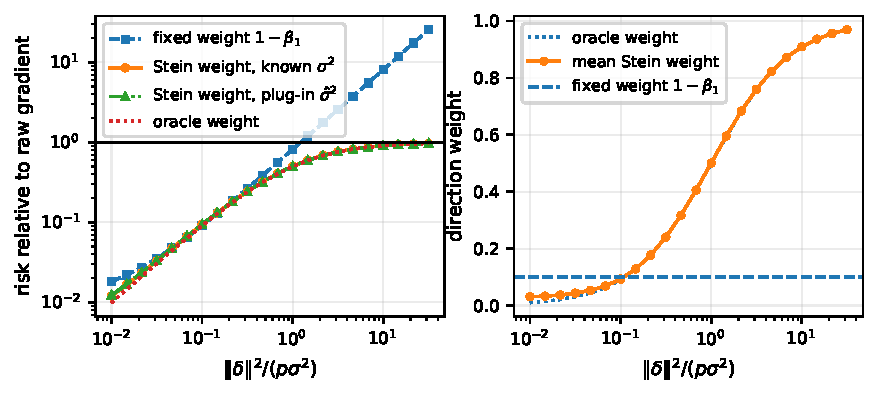
\includegraphics[width=0.92\textwidth]{sim_risk_snr.pdf}
\caption{Conditional risk relative to the raw mini-batch gradient, left, and the direction weight, right, against the signal-to-noise ratio $\|\bm\delta\|^2/(p\sigma^2)$ for $p=500$.}
\label{fig:risk_snr}
\end{figure}

\begin{table}% CAS uses key-value options here (default pos=t)
\centering
\caption{Conditional risk relative to the raw mini-batch gradient, and direction weights, at selected signal-to-noise ratios. Each entry is an average over $2\times10^{5}$ replicates.}
\label{tab:risk_snr}
\begin{tabular}{lccccc}
\toprule
 & \multicolumn{3}{c}{relative risk} & \multicolumn{2}{c}{weight} \\
\cmidrule(lr){2-4}\cmidrule(lr){5-6}
$\|\bm\delta\|^2/(p\sigma^2)$ & fixed $1-\beta_1$ & Stein & oracle & oracle & Stein \\
\midrule
0.010  & 0.018  & 0.012 & 0.010 & 0.010 & 0.031 \\
0.100  & 0.091  & 0.094 & 0.091 & 0.091 & 0.093 \\
0.464  & 0.386  & 0.320 & 0.317 & 0.317 & 0.317 \\
1.000  & 0.820  & 0.503 & 0.500 & 0.500 & 0.500 \\
3.162  & 2.571  & 0.761 & 0.760 & 0.760 & 0.760 \\
10.000 & 8.111  & 0.910 & 0.909 & 0.909 & 0.909 \\
31.623 & 25.623 & 0.970 & 0.969 & 0.969 & 0.969 \\
\bottomrule
\end{tabular}
\end{table}

\subsection{The variance estimator}

Fix $p=2048$ coordinates with variances drawn uniformly on $[0.5,2]$, run the moment recursions \eqref{eq:moments} with $\beta_1=0.9$ and $\beta_2=0.999$ over $400$ independent replicates, and compare the uncorrected statistic with the corrected one \eqref{eq:debiased}. Figure \ref{fig:variance} plots both, divided by the truth. The uncorrected statistic starts at half the truth at $t=2$ and settles at $2\beta_1/(1+\beta_1)=0.9474$, matching the closed form of Theorem \ref{thm:variance_bias} to four decimal places at every iteration, and the corrected statistic sits on one throughout. Table \ref{tab:variance} gives the numbers alongside the closed form of Theorem \ref{thm:variance_bias}.

\begin{figure}% CAS uses key-value options here (default pos=t)
\centering
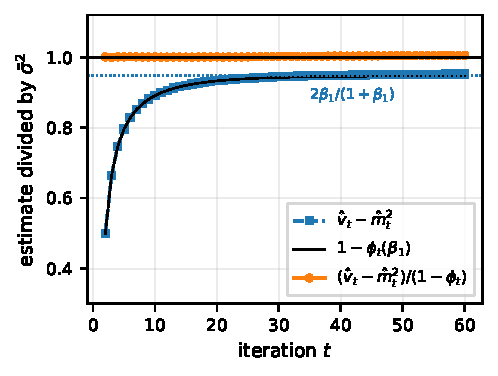
\includegraphics[width=0.48\textwidth]{sim_variance_bias.pdf}
\caption{Moment-based variance estimates divided by the true average variance, against iteration, for $p=2048$ coordinates and $400$ replicates.}
\label{fig:variance}
\end{figure}

\begin{table}% CAS uses key-value options here (default pos=t)
\centering
\caption{Moment-based variance estimates divided by the true average variance, averaged over $400$ replicates with $p=2048$ coordinates. The last column is the closed form $1-\phi_t(\beta_1)$ of Theorem \ref{thm:variance_bias}. The algorithm additionally clips the statistic at zero, which raises the uncorrected value slightly at larger $t$, to $0.9492$ at $t=40$ and $0.9523$ at $t=60$.}
\label{tab:variance}
\begin{tabular}{lccc}
\toprule
$t$ & uncorrected & corrected & $1-\phi_t(0.9)$ \\
\midrule
2   & 0.4989 & 1.0005 & 0.4986 \\
3   & 0.6641 & 0.9998 & 0.6642 \\
5   & 0.7964 & 1.0010 & 0.7956 \\
10  & 0.8915 & 1.0005 & 0.8910 \\
20  & 0.9326 & 0.9998 & 0.9328 \\
40  & 0.9457 & 0.9999 & 0.9458 \\
60  & 0.9471 & 0.9999 & 0.9472 \\
$\infty$ & 0.9474 & 1.0000 & 0.9474 \\
\bottomrule
\end{tabular}
\end{table}

\subsection{Heteroscedasticity and the loss weighting}

This study makes Corollary \ref{cor:cases} visible. Set $p=400$ and $\sigma^2_j\propto j^{-\alpha}$ normalised to unit mean, which sweeps the effective dimension from $400$ down to $1.2$ as $\alpha$ runs from $0$ to $3$. Three rules are compared under the standardised loss, namely a single pooled scalar variance with $c=p-2$, the coordinatewise rule with $c=p-2$, and the coordinatewise rule with the conservative constant $c=\peff-2$. The signal is held at three levels of $\|\bm\delta\|^2_{\bm\Sigma^{-1}}/p$.

Figure \ref{fig:effdim} reports the result and Table \ref{tab:effdim} gives the extremes. The coordinatewise rule with $c=p-2$ reduces risk uniformly, at every effective dimension and every signal level, which is Corollary \ref{cor:cases}(iii). The pooled rule is competitive when the signal is weak but fails when it is not, reaching a relative risk of $2.56$ at $\peff=1.41$ and $\|\bm\delta\|^2_{\bm\Sigma^{-1}}/p=4$. The conservative constant is safe everywhere but forfeits most of the available reduction once $\peff$ falls below about ten. The practical reading is that coordinatewise whitening, rather than any restriction of the shrinkage constant, is what neutralises heteroscedasticity.

\begin{figure}% CAS uses key-value options here (default pos=t)
\centering
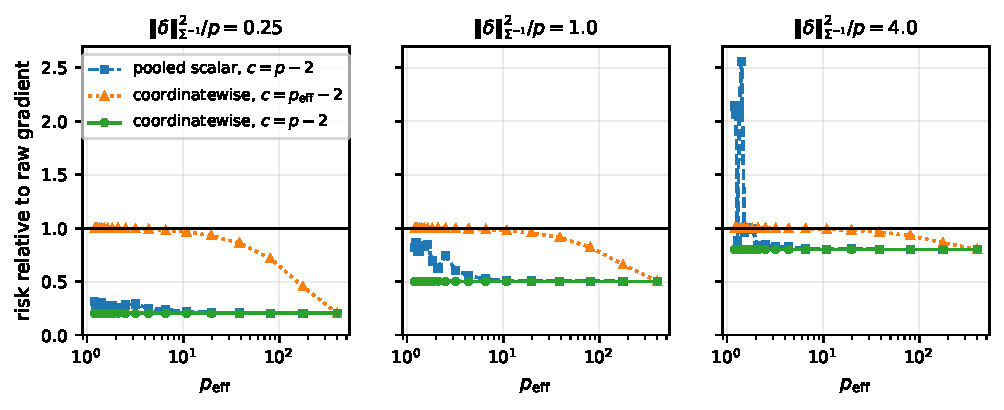
\includegraphics[width=0.98\textwidth]{sim_effective_dimension.pdf}
\caption{Risk under the standardised loss, relative to the raw gradient, against the effective dimension, for three shrinkage rules and three signal levels, with $p=400$.}
\label{fig:effdim}
\end{figure}

\begin{table}% CAS uses key-value options here (default pos=t)
\centering
\caption{Risk under the standardised loss relative to the raw gradient, at the two ends of the heteroscedasticity range, for $p=400$ and $\|\bm\delta\|^2_{\bm\Sigma^{-1}}/p=4$.}
\label{tab:effdim}
\begin{tabular}{lccc}
\toprule
$\peff$ & pooled scalar, $c=p-2$ & coordinatewise, $c=p-2$ & coordinatewise, $c=\peff-2$ \\
\midrule
400.0 & 0.802 & 0.802 & 0.802 \\
19.7  & 0.808 & 0.801 & 0.983 \\
3.19  & 0.828 & 0.802 & 0.999 \\
1.64  & 1.008 & 0.802 & 1.000 \\
1.41  & 2.561 & 0.802 & 1.000 \\
1.20  & 2.144 & 0.802 & 1.000 \\
\bottomrule
\end{tabular}
\end{table}

\subsection{Heavy-tailed gradient noise}

Draw $\bm Y$ from a multivariate Student law with $\nu$ degrees of freedom in $p=300$ dimensions, calibrate the rule to the marginal variance as Corollary \ref{cor:student} describes, and evaluate the risk for three values of the safety factor $\rho$. Figure \ref{fig:heavy} and Table \ref{tab:heavy} report the outcome. The rule with $\rho=1$ reduces risk at every $\nu$ examined, down to $\nu=3$, so the requirement $\nu>4$ that Corollary \ref{cor:student} imposes is sufficient rather than necessary, as one expects from a bound derived through a worst-case inequality. Reducing $\rho$ buys margin at a cost in risk reduction, and there is no setting in this study in which it pays.

\begin{figure}% CAS uses key-value options here (default pos=t)
\centering
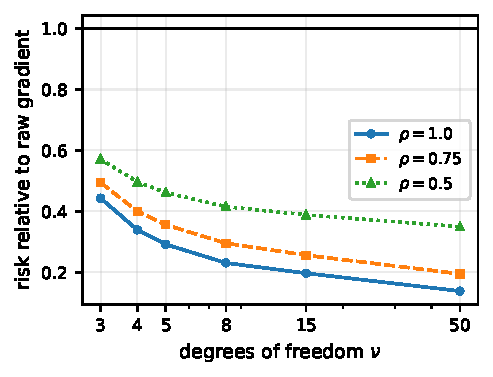
\includegraphics[width=0.48\textwidth]{sim_heavy_tails.pdf}
\caption{Risk relative to the raw gradient under multivariate Student gradient noise, against the degrees of freedom, for three safety factors, with $p=300$.}
\label{fig:heavy}
\end{figure}

\begin{table}% CAS uses key-value options here (default pos=t)
\centering
\caption{Risk relative to the raw gradient under multivariate Student gradient noise with $p=300$.}
\label{tab:heavy}
\begin{tabular}{lccc}
\toprule
$\nu$ & $\rho=1.00$ & $\rho=0.75$ & $\rho=0.50$ \\
\midrule
3  & 0.443 & 0.494 & 0.571 \\
4  & 0.339 & 0.400 & 0.497 \\
5  & 0.292 & 0.356 & 0.462 \\
8  & 0.231 & 0.295 & 0.415 \\
15 & 0.197 & 0.256 & 0.388 \\
50 & 0.138 & 0.195 & 0.349 \\
\bottomrule
\end{tabular}
\end{table}

\subsection{Optimisation under controlled noise}
\label{sec:sim_opt}

The studies above concern estimation risk. Whether a lower estimation risk produces a better optimiser is a separate question, and this study addresses it on two problems in which the noise level can be set directly.

The first is a quadratic objective in $p=400$ dimensions with diagonal curvature spread over $[0.05,2]$, observed through gradients corrupted by isotropic noise of scale $\tau$. The second is multinomial logistic regression in $200$ features and ten classes with $N=20\,000$ observations, mini-batches of $64$, and a controlled rate of label flips. Four optimisers are compared at their own tuned step sizes, over five seeds and $3000$ steps on the quadratic and three seeds and $2000$ steps on the logistic problem, and the reported comparison against AdamW is paired by seed.

Table \ref{tab:opt_noise} and Figure \ref{fig:noise} give the results. With the step sizes tuned, the ranking on the quadratic is set by the noise scale rather than being uniform. SR-Adam's terminal objective is $32$ and $9$ per cent below AdamW's at $\tau=0.1$ and $\tau=0.25$, and $27$ and $24$ per cent below at $\tau=2$ and $\tau=4$, but it is $11$ and $30$ per cent above at $\tau=0.5$ and $\tau=1$. On the logistic problem it is between $4$ and $5$ per cent below AdamW up to a flip rate of $0.2$ and \rev{about} $5$ per cent above at flip rates $0.3$ and $0.4$, where the tuned AdamW step size is three times smaller than at the lower flip rates. All eleven paired differences are significant at conventional levels, with $|t|$ between $4.0$ and $27.6$, so the reversal is not sampling noise. Tuning also changes the position of plain momentum SGD: it is competitive on the clean logistic problem ($0.233$ against AdamW's $0.244$) and remains far behind on the ill-conditioned quadratic, as expected.

\begin{figure}% CAS uses key-value options here (default pos=t)
\centering
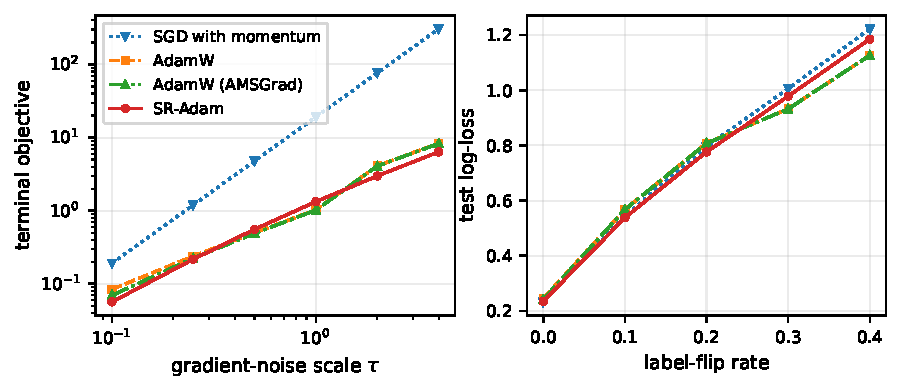
\includegraphics[width=0.92\textwidth]{sim_noise_levels.pdf}
\caption{Terminal objective on the noisy quadratic, left, and test log-loss on the logistic problem with label noise, right.}
\label{fig:noise}
\end{figure}

\begin{table}% CAS uses key-value options here (default pos=t)
\centering
\caption{Optimisation under controlled noise at per-optimiser tuned step sizes. The quadratic panel reports the terminal objective over five seeds and $3000$ steps, the logistic panel the test log-loss over three seeds and $2000$ steps. The last column is the paired difference between AdamW and SR-Adam with its $t$ statistic.}
\label{tab:opt_noise}
\footnotesize\setlength{\tabcolsep}{3.5pt}
\begin{tabular}{lccccr}
\toprule
 & SGD, momentum & AdamW & AMSGrad & SR-Adam & paired diff ($t$) \\
\midrule
\multicolumn{6}{l}{Noisy quadratic, gradient-noise scale $\tau$} \\
$\tau=0.10$ & 0.191 & 0.084 & 0.069 & 0.057 & $+0.027$ $(9.0)$ \\
$\tau=0.25$ & 1.193 & 0.238 & 0.224 & 0.216 & $+0.022$ $(4.0)$ \\
$\tau=0.50$ & 4.773 & 0.500 & 0.488 & 0.555 & $-0.055$ $(-4.4)$ \\
$\tau=1.00$ & 19.090 & 1.025 & 1.017 & 1.328 & $-0.303$ $(-26.9)$ \\
$\tau=2.00$ & 76.361 & 4.093 & 4.071 & 2.983 & $+1.110$ $(27.6)$ \\
$\tau=4.00$ & 305.443 & 8.319 & 8.277 & 6.361 & $+1.958$ $(20.2)$ \\
\midrule
\multicolumn{6}{l}{Logistic regression, label-flip rate} \\
0.0 & 0.233 & 0.244 & 0.242 & 0.235 & $+0.010$ $(18.4)$ \\
0.1 & 0.544 & 0.568 & 0.567 & 0.538 & $+0.030$ $(12.8)$ \\
0.2 & 0.796 & 0.808 & 0.808 & 0.777 & $+0.031$ $(16.2)$ \\
0.3 & 1.006 & 0.933 & 0.933 & 0.979 & $-0.046$ $(-8.1)$ \\
0.4 & 1.222 & 1.127 & 1.127 & 1.185 & $-0.058$ $(-9.4)$ \\
\bottomrule
\end{tabular}
\end{table}

\subsection{The bias floor and the batch size}

Proposition \ref{prop:batch} predicts that the floor in \eqref{eq:conv_bound} is inversely proportional to the batch size. To test it, a two-layer network with $120$ inputs, $48$ hidden units and eight classes is fitted to synthetic data from a fixed teacher, at seven batch sizes from eight to $512$, over five seeds, with the realised $\tr\widehat{\bm\Sigma}_t$ recorded along each run. The trace is reported rather than the floor $c_t\lambda_{\max}(\widehat{\bm\Sigma}_t)$ itself, since the two scale with the batch size in the same way and the trace is the less noisy summary. Table \ref{tab:batch} and Figure \ref{fig:batch} report the outcome. The noise trace falls by a factor of $1.86$ on average for each doubling of the batch, against the predicted factor of two, and the realised Stein weight stays near the fixed Adam weight, varying between $0.13$ and $0.16$. The terminal training losses of the two optimisers differ by less than $0.01$ at every batch size, with SR-Adam ahead at the three smallest batch sizes, only marginally so at $B=32$, and behind at the four largest.

That last finding should be read carefully. At $B=8$ and at $B=32$ the difference is not statistically significant, with $|t|$ of $2.7$ and $1.9$ below the two-sided $5$ per cent critical value of $2.78$ on four degrees of freedom; at $B=16$ it is significant, but the margin is only $0.0032$ in training loss. At the four largest batch sizes the difference is significant but very small, from $0.0012$ to $0.0080$ in training loss, and it favours AdamW. The sign of the difference reverses around a batch size of $32$. In particular it gives no support to a large-batch advantage for the method, and none is claimed.

\begin{figure}% CAS uses key-value options here (default pos=t)
\centering
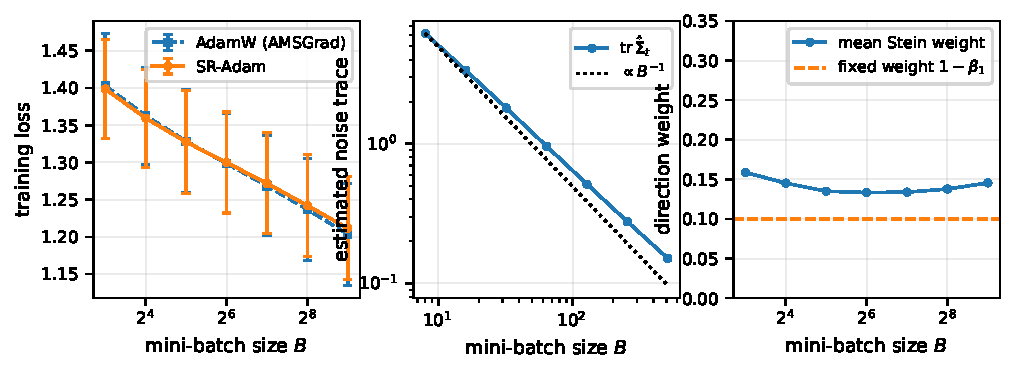
\includegraphics[width=0.98\textwidth]{sim_batch_size.pdf}
\caption{Terminal training loss, left, realised gradient-noise trace, centre, and realised direction weight, right, against mini-batch size, over five seeds.}
\label{fig:batch}
\end{figure}

\begin{table}% CAS uses key-value options here (default pos=t)
\centering
\caption{Batch-size study over five seeds. Losses are means with standard deviations across seeds; the paired difference is AdamW minus SR-Adam with its $t$ statistic.}
\label{tab:batch}
\begin{tabular}{lccrcc}
\toprule
$B$ & AdamW (AMSGrad) & SR-Adam & paired diff ($t$) & $\tr\widehat{\bm\Sigma}_t$ & Stein weight \\
\midrule
8   & $1.4030\pm0.0702$ & $1.3987\pm0.0670$ & $+0.0042$ $(2.7)$    & 6.163 & 0.159 \\
16  & $1.3627\pm0.0650$ & $1.3595\pm0.0656$ & $+0.0032$ $(7.1)$    & 3.357 & 0.145 \\
32  & $1.3285\pm0.0693$ & $1.3275\pm0.0690$ & $+0.0010$ $(1.9)$    & 1.806 & 0.135 \\
64  & $1.2988\pm0.0674$ & $1.2999\pm0.0678$ & $-0.0012$ $(-4.6)$   & 0.961 & 0.133 \\
128 & $1.2685\pm0.0672$ & $1.2718\pm0.0678$ & $-0.0033$ $(-6.3)$   & 0.513 & 0.134 \\
256 & $1.2368\pm0.0682$ & $1.2422\pm0.0689$ & $-0.0054$ $(-8.2)$   & 0.276 & 0.138 \\
512 & $1.2035\pm0.0689$ & $1.2115\pm0.0692$ & $-0.0080$ $(-18.7)$  & 0.151 & 0.146 \\
\bottomrule
\end{tabular}
\end{table}

\subsection{Verification of the analytical constants}

Every constant asserted in Sections \ref{sec:risk} to \ref{sec:convergence} was checked against a Monte Carlo evaluation before being written down. The identity \eqref{eq:master_identity} agrees with a direct evaluation of the risk difference to within four combined standard errors at $3\times10^{6}$ replicates. The empirical sign change of the risk difference lies at or beyond the upper endpoint of \eqref{eq:master_window} in every configuration tested, confirming that the window is sufficient and, in the heteroscedastic case, conservative. The threshold in Corollary \ref{cor:twofold} is located between $\hat\sigma^2=1.95$ and $\hat\sigma^2=2.05$. The displacement bound \eqref{eq:displacement} is attained to six decimal places. The closed form \eqref{eq:variance_bias} agrees with the simulated bias at every iteration examined, and the pooled variance estimator has standard deviation proportional to $p^{-1/2}$ across a $256$-fold range of $p$, with the product $p^{1/2}\,\mathrm{sd}$ varying by a factor of $1.12$.

%%%%%%%%%%%%%%%%%%%%%%%%%%%%%%%%%%%%%%%%%%%%%%%%%%%%%%%%%%%%%%%%%%%%%%%
%% Empirical evaluation — code provenance (not printed)
%%   sec:experiments intro     : code/sr_adam.py, code/path4_dim_sweep.py, ...
%%   tab:dim_sweep             : code/path4_dim_sweep.py -> out/path4_dim_sweep.json
%%   tab:dim_sweep_common      : code/path4_dim_sweep.py --common-lr
%%                               -> out/path4_dim_sweep_common.json (protocol ablation)
%%   tab:reg (tab_regression)  : code/paper_tables.py -> paper/tab_regression.tex
%%                               (datasets: diabetes, california_housing, wine_quality,
%%                                linnerud, protein, blogfeedback; linear + MLP)
%%   tab:clf (tab_classification): code/paper_tables.py -> paper/tab_classification.tex
%%                               + code/gnn_pilot.py / gnn_pilot_planetoid.py (GCN rows)
%%   tab:noise (tab_noise)     : code/noise_sweep.py -> paper/tab_noise.tex
%%   fig:noise_sweep           : code/noise_sweep.py -> paper/fig_noise_sweep.pdf
%%   fig:gnn_acc               : code/make_paper_barfigs.py (from gnn_pilot_*.json)
%%   fig:regime_win            : code/make_paper_barfigs.py
%%   raw JSON                  : out/path4_dim_sweep.json, out/path4_dim_sweep_common.json,
%%                               out/paper_tables.json,
%%                               out/noise_sweep.json, out/gnn_pilot_*.json
%%   driver scripts            : scripts/run_paper_tables.sh, scripts/run_grouping_grid.sh
%%%%%%%%%%%%%%%%%%%%%%%%%%%%%%%%%%%%%%%%%%%%%%%%%%%%%%%%%%%%%%%%%%%%%%
\section{Empirical evaluation}
\label{sec:experiments}

This section asks where the risk-optimal weight improves on Adam-type methods on problems outside the Monte Carlo designs of Section \ref{sec:simulation}. The code base, the optimiser interfaces, and the seed schedule are held fixed; only the optimiser and the problem change. Baselines are SGD with momentum, AdamW \citep{loshchilov2019}, and AdamW with the AMSGrad preconditioner \citep{reddi2018}. Unless stated otherwise, SR-Adam uses the defaults of Algorithm \ref{alg:sradam} ($\rho=1$, $\omega=0.1$, $\gamma=1$, $\tau=5$) and the comparison is paired by seed on the final test loss or accuracy. Implementations accompany the paper.

Every baseline below is tuned rather than left at a common step size, with one deliberate exception: Table \ref{tab:dim_sweep_common} repeats the dimension sweep under the shared default step size, as an ablation of the comparison itself in the last subsection of this section. Each optimiser receives its own grid of three to five candidate step sizes spanning one to two orders of magnitude, scored on two tuning seeds --- held-out validation loss on the logistic and graph pilots, terminal loss elsewhere --- and the reported run then uses the study's seed set shared across optimisers. The number of pilots varies: the controlled study of Section \ref{sec:sim_opt} retunes at every noise level, while the dimension sweep and the tabular studies tune once per problem family on a single representative pilot (the quadratic at $\tau=1$ at the smallest $p$) and reuse that choice across the family --- the two exceptions are the $\tau=4$ and flip-rate-$0.4$ columns of Table \ref{tab:dim_sweep}, which are tuned at their own noise level. The graph-network pilots in Table \ref{tab:clf} are tuned per dataset on a grid of five step sizes from $10^{-3}$ to $10^{-1}$, identical for both optimisers, scored on validation accuracy at clean labels, and the chosen step size is reused at both label-noise levels. The full grid tables are stored with the results so that the protocol is auditable. Two diagnostics are recorded alongside these runs. The mean per-step wall-clock time was $0.55$\,ms on the $p=400$ quadratic under Gaussian noise ($0.90$\,ms under Student-$t$ noise) and $1.8$\,ms on the $200$-feature logistic problem, averaged over the three optimisers of the sweep, so the three extra reductions of Section \ref{sec:algorithm} are not a visible share of the step. The gate of Remark \ref{rem:gate} is recorded as the fraction of parameter blocks on which it is open at the last step of a run: it was open on every block at the end of every run in Table \ref{tab:opt_noise} and on Digits, while on the remaining tabular problems it ranges from none of the blocks to three quarters, a block of dimension three or less being unable to open it. Where it is closed the block falls back to the Adam weight, so the safeguard does fire on some of these problems.

\paragraph{Data and tasks}
Three families are used. (i)~\emph{Public tabular regression}: Diabetes, California Housing, Wine Quality, Linnerud, and BlogFeedback (UCI/OpenML or scikit-learn; linear model and a one-hidden-layer MLP). (ii)~\emph{Classification}: handwritten digits, breast cancer, ionosphere, and iris (logistic regression and a small MLP), together with node classification on the Planetoid graphs Cora, CiteSeer, and PubMed (two-layer GCN \citep{kipf2017}), with optional training-label noise. (iii)~\emph{Synthetic controlled noise} (no external dataset): a quadratic with diagonal curvature and additive Gaussian or Student-$t$ gradient noise, and multinomial logistic regression with a controlled label-flip rate; the last subsection studies families (ii) and (iii) under label noise, dimension growth and the two step-size protocols. 

\subsection{Real regression}
%% code: paper_tables.py (loaders in path3_uci.py / path6_year_blog_clf.py)

Table \ref{tab:reg} reports public regression sets. For each dataset we fit (i) a linear model and (ii) a one-hidden-layer multilayer perceptron (MLP) with a nonlinear activation; features and targets are standardised on the training split. The entry is the paired gap in test MSE, AdamW minus SR-Adam (positive favours SR-Adam).

The linear rows all favour SR-Adam: the largest is BlogFeedback ($p=280$) at $+1.21$, and the remaining four lie between $+0.003$ and $+0.025$. The MLP rows are mixed, three of them favouring SR-Adam and two against, with the largest single gain on Diabetes ($+0.47$). That split is expected rather than contradictory. A linear least-squares problem is convex and the search direction is a noisy estimate of a well-defined gradient, which is the setting of Sections \ref{sec:risk} and \ref{sec:variance}. A one-hidden-layer MLP is already non-convex: the Stein weight shrinks the current gradient toward a historical average, which helps when that average is a good proxy for the population gradient and can hurt when the loss landscape forces frequent changes of direction. In addition, the MLP is more parameterised than the linear model on the same $n$ and $p$, so the blockwise variance estimates that drive $k_t$ are noisier. We therefore read the linear rows as the primary regression evidence and the MLP rows as a mild nonlinearity check.

%% Table tab:reg: code/paper_tables.py -> paper/tab_regression.tex (out/paper_tables.json)
\begin{table}% CAS uses key-value options here (default pos=t)
\centering
\caption{Regression on public tabular sets. Gap in test MSE, AdamW minus SR-Adam; bold positive entries favour SR-Adam. \emph{Model} is either a linear regressor or a one-hidden-layer MLP (nonlinear).}
\label{tab:reg}
% Auto-generated by paper_tables.py � do not edit by hand
\begin{tabular}{llrrc}
\toprule
Dataset & Model & $n$ & $p$ & Gap (MSE) \\
\midrule
% Model: linear = linear regressor; MLP = one hidden layer, nonlinear
Diabetes & linear & 442 & 10 & $\bm{+0.003}$ \\
Diabetes & MLP & 442 & 10 & $\bm{+0.466}$ \\
California Housing & linear & 20640 & 8 & $\bm{+0.023}$ \\
California Housing & MLP & 20640 & 8 & $-0.003$ \\
Wine Quality & linear & 1599 & 11 & $\bm{+0.014}$ \\
Wine Quality & MLP & 1599 & 11 & $\bm{+0.067}$ \\
Linnerud & linear & 20 & 3 & $\bm{+0.025}$ \\
Linnerud & MLP & 20 & 3 & $-0.308$ \\
BlogFeedback & linear & 8000 & 280 & $\bm{+1.209}$ \\
BlogFeedback & MLP & 8000 & 280 & $\bm{+0.041}$ \\
\bottomrule
\end{tabular}

\end{table}

\subsection{Classification}
%% code: paper_tables.py (tabular/digits); gnn_pilot.py, gnn_pilot_planetoid.py (GCN)

Table \ref{tab:clf} covers logistic regression, a small MLP, and a two-layer graph convolutional network \citep{kipf2017} on clean labels. Test accuracy is reported for AdamW and SR-Adam; the better entry is bolded. SR-Adam is ahead on Breast Cancer, Ionosphere and all three graphs, and marginally behind on Digits and Iris. The largest margin is Ionosphere ($+2.3$ points), where the number of features is comparable to the sample size; on the graphs the margins are at most a third of a point at the tuned step sizes, and on PubMed the two agree to four hundredths of a point.

%% Table tab:clf: code/paper_tables.py -> paper/tab_classification.tex
%%   GCN rows from paper_tables.gnn_rows() at the step sizes chosen by the
%%   per-dataset grids of gnn_pilot.py / gnn_pilot_planetoid.py (--tune)
%%   recorded in out/gnn_{cora,citeseer,pubmed}_tune.json
\begin{table}% CAS uses key-value options here (default pos=t)
\centering
\caption{Classification test accuracy (per cent), clean training labels. Models: logistic regression, one-hidden-layer MLP, and GCN \citep{kipf2017}. Bold $=$ higher accuracy.}
\label{tab:clf}
% Auto-generated by paper_tables.py � do not edit by hand
\begin{tabular}{llrrccc}
\toprule
Dataset & Model & $n$ & $p$ & $K$ & AdamW & SR-Adam \\
\midrule
Digits & logistic & 1797 & 64 & 10 & 95.9 & 95.8 \\
Breast Cancer & logistic & 569 & 30 & 2 & 96.1 & \textbf{97.4} \\
Breast Cancer & MLP & 569 & 30 & 2 & 96.6 & \textbf{97.5} \\
Ionosphere & logistic & 351 & 34 & 2 & 86.5 & \textbf{88.8} \\
Iris & logistic & 150 & 4 & 3 & 95.1 & 94.2 \\
Cora & GCN & 2708 & 1433 & 7 & 78.6 & \textbf{78.9} \\
CiteSeer & GCN & 3327 & 3703 & 6 & 64.7 & \textbf{65.0} \\
PubMed & GCN & 19717 & 500 & 3 & 76.6 & \textbf{76.6} \\
\bottomrule
\end{tabular}

\end{table}

\subsection{Ablation study}
This subsection isolates the two factors the method is sensitive to, one problem-side and one method-side: the noise that corrupts the data, and the step-size protocol used to compare against AdamW. Both use the paired protocol of this section.
\subsubsection{Label noise}
%% code: noise_sweep.py (classification + target-noise regression)

Table \ref{tab:noise} and Figure \ref{fig:noise_sweep} isolate the effect of corrupting training labels or targets, with the regression block first (matching Tables~\ref{tab:reg}--\ref{tab:clf}). Throughout this section the gap is signed so that positive favours SR-Adam: for classification it is test accuracy of SR-Adam minus AdamW in percentage points, and for regression it is test MSE of AdamW minus SR-Adam. On Digits with multinomial logistic regression the ranking reverses as soon as labels are corrupted: clean labels give a gap of $-1.3$ points, and with label-noise rates from $10$ to $50$ per cent the gap grows from $+3.9$ to $+13.5$ points, increasing with the noise rate. On a well-separated binary problem (Breast Cancer) the gap is modest and positive at every rate, from $+0.2$ to $+3.8$ points. On linear regression the pattern is weaker and not of a consistent sign: Diabetes is positive at every target-noise level ($+0.015$ to $+0.027$), Wine Quality is positive at the two lower levels and tied at the highest ($-0.001$), and California Housing is negative at the two lower levels and positive but imprecise at the highest ($+0.069$, $t=1.3$). This is the noise-dominated regime of Corollary \ref{cor:cases}: shrinkage helps when the mini-batch signal is unreliable, most clearly on the classification side, and adds little when it is not.

%% Table tab:noise: code/noise_sweep.py -> paper/tab_noise.tex (out/noise_sweep.json)
\begin{table}% CAS uses key-value options here (default pos=t)
\centering
\caption{Label (or target) noise. Upper block: linear regression with target noise on $y$ (test MSE). Lower block: classification with training-label noise (test accuracy, per cent). Gap is AdamW minus SR-Adam for MSE and SR-Adam minus AdamW for accuracy (pp); positive favours SR-Adam (bold).}
\label{tab:noise}
% Auto-generated by noise_sweep.py
\begin{tabular}{llccc}
\toprule
Problem & Noise & AdamW & SR-Adam & Gap \\
\midrule
\multicolumn{5}{l}{\emph{Regression (linear), target noise on $y$}} \\
Wine Quality (linear) & 0.0 & 0.6270 & 0.6228 & $\bm{+0.0042}$ \\
Wine Quality (linear) & 0.5 & 0.6312 & 0.6278 & $\bm{+0.0033}$ \\
Wine Quality (linear) & 1.0 & 0.6299 & 0.6309 & $-0.0010$ \\
Diabetes (linear) & 0.0 & 0.5315 & 0.5047 & $\bm{+0.0268}$ \\
Diabetes (linear) & 0.5 & 0.5263 & 0.5112 & $\bm{+0.0151}$ \\
Diabetes (linear) & 1.0 & 0.5494 & 0.5345 & $\bm{+0.0149}$ \\
California Housing (linear) & 0.0 & 0.5384 & 0.5527 & $-0.0143$ \\
California Housing (linear) & 0.5 & 0.5148 & 0.5322 & $-0.0174$ \\
California Housing (linear) & 1.0 & 0.5183 & 0.4496 & $\bm{+0.0688}$ \\
\midrule
\multicolumn{5}{l}{\emph{Classification, training-label noise}} \\
Digits (logistic) & 0.0 & 95.7 & 94.4 & $-1.3$pp \\
Digits (logistic) & 0.1 & 89.2 & 93.1 & $\bm{+3.9}$pp \\
Digits (logistic) & 0.2 & 85.5 & 90.7 & $\bm{+5.3}$pp \\
Digits (logistic) & 0.3 & 82.5 & 90.4 & $\bm{+7.9}$pp \\
Digits (logistic) & 0.5 & 72.9 & 86.4 & $\bm{+13.5}$pp \\
Breast Cancer (logistic) & 0.0 & 97.1 & 97.3 & $\bm{+0.2}$pp \\
Breast Cancer (logistic) & 0.1 & 96.1 & 96.8 & $\bm{+0.7}$pp \\
Breast Cancer (logistic) & 0.2 & 94.1 & 94.9 & $\bm{+0.8}$pp \\
Breast Cancer (logistic) & 0.3 & 94.7 & 96.4 & $\bm{+1.6}$pp \\
Breast Cancer (logistic) & 0.5 & 90.9 & 94.7 & $\bm{+3.8}$pp \\
\bottomrule
\end{tabular}

\end{table}

%% Figure fig:noise_sweep: code/noise_sweep.py -> paper/fig_noise_sweep.pdf
\begin{figure}% CAS uses key-value options here (default pos=t)
\centering
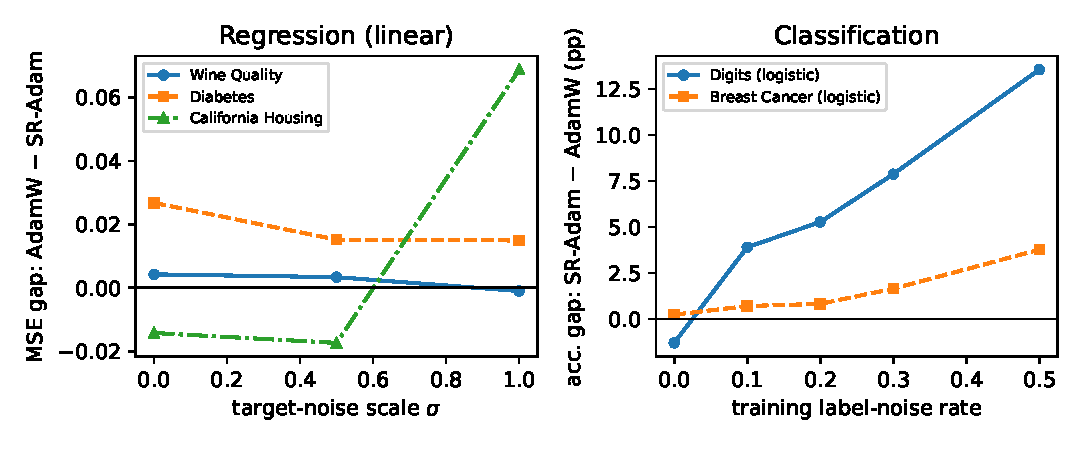
\includegraphics[width=1\textwidth]{fig_noise_sweep.pdf}
\caption{Noise and the Stein weight. Left: MSE gap (AdamW minus SR-Adam) on linear regression against target-noise scale for three tabular sets. Right: classification accuracy gap (SR-Adam minus AdamW) against training label-noise rate. Positive values favour SR-Adam. On Digits the Stein weight is ahead once labels are corrupted, by up to $+13.5$ accuracy points at a $50$ per cent flip rate; on regression the MSE gap is small and not of a consistent sign across the three sets.}
\label{fig:noise_sweep}
\end{figure}

\subsubsection{Dimension and controlled noise}
%% code: path4_dim_sweep.py  (also phase_diagram.py for the wider grid)

The controlled family isolates the high-dimensional claim of Sections \ref{sec:risk} and \ref{sec:convergence}. On a quadratic with diagonal curvature and additive gradient noise at scale $\tau$, and on multinomial logistic regression with a controlled label-flip rate, the block dimension $p$ runs over $\{10,20,50,100,200,400,500\}$. The paired gap on the terminal objective, AdamW minus SR-Adam, is recorded at $\tau\in\{0.1,1,4\}$, under Student-$t$ noise at $\tau=1$, and at label-flip rates $0.2$ and $0.4$. The step-size protocol itself is an ablation factor of this subsection, so the sweep is reported under both protocols, the shared-default one first: the step size the first version of this manuscript used --- $0.02$ on the quadratic problems and $0.03$ on the logistic problem for every optimiser, nothing tuned --- on identical seeds, step count and problem grid. Table \ref{tab:dim_sweep_common} reports that arm. The gap grows with $p$ on every column: the quadratic at $\tau=1$ runs from $+0.010$ at $p=10$ to $+0.621$ at $p=500$, Student-$t$ from $+0.006$ to $+0.400$, and the logistic problem at flip rate $0.2$ from $+0.000$ to $+1.452$, and $38$ of the $42$ settings favour SR-Adam --- the claim made by the earlier draft.

%% Table tab:dim_sweep_common: code/path4_dim_sweep.py --common-lr -> out/path4_dim_sweep_common.json
\begin{table}% CAS uses key-value options here (default pos=t)
\centering
\caption{Ablation of the step-size protocol: the dimension sweep at the shared default step size that the first version of this manuscript used --- $0.02$ on the quadratic problems and $0.03$ on the logistic problem for every optimiser, nothing tuned. Paired gap on the terminal loss, AdamW minus SR-Adam, for $p\in\{10,20,50,100,200,400,500\}$: quadratic with Gaussian gradient noise at $\tau\in\{0.1,1,4\}$, quadratic with Student-$t$ noise at $\tau=1$, and logistic label noise at flip rates $0.2$ and $0.4$; identical seeds, steps and problem grid in both protocols. Positive values favour SR-Adam; $38$ of the $42$ settings do, the four exceptions being the $\tau=4$ column at $p\in\{10,20,50,400\}$, none of them significant ($|t|\leq 1.34$).}
\label{tab:dim_sweep_common}
\footnotesize\setlength{\tabcolsep}{3.5pt}
\begin{tabular}{ccccccc}
\toprule
$p$ & \multicolumn{3}{c}{quadratic (Gaussian)} & Student-$t$ & \multicolumn{2}{c}{logistic} \\
 & $\tau{=}0.1$ & $\tau{=}1$ & $\tau{=}4$ & $\tau{=}1$ & flip $0.2$ & flip $0.4$ \\
\midrule
10  & $+0.002$ & $+0.010$ & $-0.016$ & $+0.006$ & $+0.000$ & $+0.002$ \\
20  & $+0.006$ & $+0.019$ & $-0.082$ & $+0.009$ & $+0.005$ & $+0.001$ \\
50  & $+0.013$ & $+0.037$ & $-0.143$ & $+0.038$ & $+0.020$ & $+0.018$ \\
100 & $+0.027$ & $+0.140$ & $+0.219$ & $+0.099$ & $+0.064$ & $+0.059$ \\
200 & $+0.040$ & $+0.179$ & $+0.147$ & $+0.116$ & $+0.193$ & $+0.154$ \\
400 & $+0.095$ & $+0.521$ & $-0.395$ & $+0.339$ & $+0.838$ & $+0.588$ \\
500 & $+0.111$ & $+0.621$ & $+0.383$ & $+0.400$ & $+1.452$ & $+1.049$ \\
\bottomrule
\end{tabular}
\end{table}

Table \ref{tab:dim_sweep} repeats the sweep with the step sizes tuned per optimiser (the quadratic grid chosen at $\tau=1$ and reused at $\tau=0.1$ and under Student-$t$ noise, the logistic grid at flip rate $0.2$; the $\tau=4$ and flip-rate-$0.4$ columns are tuned at their own noise level). Under that protocol the sign of the gap is set by the noise level and not by the dimension --- exactly the regime statement of the risk analysis. SR-Adam wins at every $p$ at $\tau=0.1$ and at flip rate $0.4$, and at $\tau=4$ the gap turns positive at $p\in\{100,200,500\}$; a tuned AdamW is ahead only in the intermediate band ($\tau=1$, Student-$t$ at $\tau=1$, flip rate $0.2$). Seventeen of the forty-two settings favour SR-Adam, and every one of them sits at an end of the noise axis. The heavy label-noise column is the strongest evidence in the table: the paired gap grows with $p$ from $+0.015$ at $p=10$ to $+4.13$ at $p=500$ --- per coordinate from $7\times10^{-4}$ at $p=20$ to $8\times10^{-3}$ at $p=500$, an order of magnitude --- with $|t|$ between $10.5$ and $47.7$ at every $p\geq 50$. This is the corruption-dominated regime in which the risk-optimal weight departs furthest from any fixed momentum weight, and there the advantage does grow with the block dimension. The sign at this flip rate does not contradict Table \ref{tab:opt_noise}, where a tuned AdamW is a few per cent ahead at flip rates $0.3$ and $0.4$: that study trains on $N=20\,000$ points for $2000$ steps while this sweep trains on $N=4000$ for $800$, so per coordinate the sweep is the far more estimation-limited problem --- the two results place the crossover on the same axis, the variance of the gradient estimate per coordinate, rather than on the flip rate alone. At $\tau=0.1$ the per-coordinate gap stays flat ($3\times10^{-6}$ to $1.2\times10^{-4}$), so the growing component appears only once the noise clearly corrupts the signal.

%% Table tab:dim_sweep: code/path4_dim_sweep.py -> out/path4_dim_sweep.json
\begin{table}% CAS uses key-value options here (default pos=t)
\centering
\caption{The same sweep as Table \ref{tab:dim_sweep_common} --- same problems, noise levels, $p$ grid, seeds, steps and problem grid --- with the step sizes tuned per optimiser: the quadratic grid is chosen at $\tau=1$ and reused at $\tau=0.1$ and under Student-$t$ noise, and the logistic grid at flip rate $0.2$, while the $\tau=4$ and flip-rate-$0.4$ columns are tuned at their own noise level. Paired gap on the terminal loss, AdamW minus SR-Adam; positive values favour SR-Adam.}
\label{tab:dim_sweep}
\footnotesize\setlength{\tabcolsep}{3.5pt}
\begin{tabular}{ccccccc}
\toprule
$p$ & \multicolumn{3}{c}{quadratic (Gaussian)} & Student-$t$ & \multicolumn{2}{c}{logistic} \\
 & $\tau{=}0.1$ & $\tau{=}1$ & $\tau{=}4$ & $\tau{=}1$ & flip $0.2$ & flip $0.4$ \\
\midrule
10  & $+0.000$ & $-0.007$ & $-0.016$ & $-0.001$ & $-0.005$ & $+0.015$ \\
20  & $+0.002$ & $-0.028$ & $-0.082$ & $-0.009$ & $-0.014$ & $+0.013$ \\
50  & $+0.001$ & $-0.054$ & $-0.143$ & $-0.013$ & $-0.023$ & $+0.100$ \\
100 & $+0.005$ & $-0.019$ & $+0.219$ & $-0.003$ & $-0.062$ & $+0.237$ \\
200 & $+0.001$ & $-0.156$ & $+0.147$ & $-0.062$ & $-0.144$ & $+0.764$ \\
400 & $+0.012$ & $-0.237$ & $-0.395$ & $-0.067$ & $-0.572$ & $+2.349$ \\
500 & $+0.007$ & $-0.216$ & $+0.383$ & $-0.075$ & $-0.919$ & $+4.132$ \\
\bottomrule
\end{tabular}
\end{table}

The two protocols differ in exactly twenty-one cells, and those cells are precisely the intermediate band ($\tau=1$, Student-$t$ at $\tau=1$, flip rate $0.2$). The mechanism is visible in the chosen values: halving the step size there takes AdamW from $0.02$ to $0.01$ on the quadratic and from $0.03$ to $0.01$ on the logistic problem, while SR-Adam keeps the value the shared default already gave it ($0.02$ and $0.03$) --- the common step size of the earlier draft was in effect SR-Adam's own tuned step size. Both ends of the noise axis give the same outcome under the two protocols (all seven cells at $\tau=0.1$, all seven at flip rate $0.4$, and the same three cells at $\tau=4$\rev{; the $\tau=4$ column is in fact identical in the two tables, because tuning at that noise level returned the shared default step size for both optimisers}), so the regime structure is a property of the problem and not of the comparison, while the size of the deficit at intermediate noise is a property of the baseline. Table \ref{tab:dim_sweep} is therefore the fair comparison and the headline of this subsection, and Table \ref{tab:dim_sweep_common} the ablation of the comparison itself.

%\clearpage
%\newpage 

\clearpage

%% Figure fig:regime_win: code/make_paper_barfigs.py (fractions from out/*.json)
\begin{figure}% CAS uses key-value options here (default pos=t)
\centering
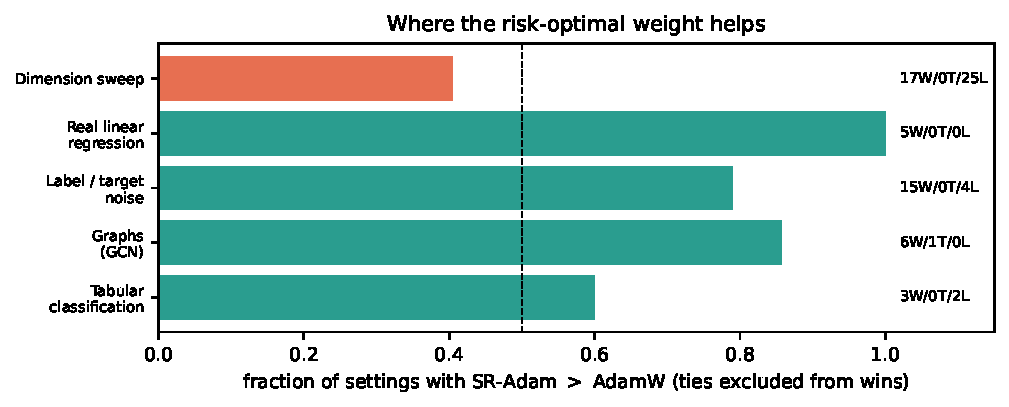
\includegraphics[width=0.9\textwidth]{regime_winrate.pdf}
\caption{Fraction of settings in which SR-Adam beats AdamW, ties excluded, by problem family, at the per-optimiser tuned step sizes: dimension sweep ($17/42$\rev{, the cell printed as $+0.000$ in Table \ref{tab:dim_sweep} being positive before rounding}), real linear regression ($5/5$), label and target noise ($15/19$), graph node classification ($6/7$, one tie), and clean tabular classification ($3/5$).}
\label{fig:regime_win}
\end{figure}



Across these families the risk-optimal weight helps when the problem is estimation-heavy and the gradient noise is either small relative to the curvature or clearly corrupting the signal. Figure \ref{fig:regime_win} summarises the same evidence as a win rate. Every linear regression cell, fifteen of the nineteen label and target noise cells, six of the seven graph cells and both ends of the noise axis of the dimension sweep --- every cell at $\tau=0.1$ and at flip rate $0.4$, and three of the four largest blocks at $\tau=4$ --- favour SR-Adam; at the intermediate noise scales of the controlled study, at $\tau=1$ and moderate label noise in the sweep, and on clean tabular classification a tuned AdamW matches or beats it. Normalised by the dimension the gap stays flat at $\tau=0.1$ but grows with $p$ from $7\times10^{-4}$ to $8\times10^{-3}$ under heavy label noise (Table \ref{tab:dim_sweep}), so the sweep supports a noise-robust advantage that becomes dimension-dependent once the noise dominates the signal, rather than a uniform one. Together with the risk theory of Sections \ref{sec:risk}--\ref{sec:variance} this is a coherent picture, and it is not a claim of universal optimiser dominance.

%%%%%%%%%%%%%%%%%%%%%%%%%%%%%%%%%%%%%%%%%%%%%%%%%%%%%%%%%%%%%%%%%%%%%%
\section{Discussion}
\label{sec:conclusion}

The search direction of an adaptive gradient method is a shrinkage estimator of the population gradient whose weight is set by a hyperparameter. Replacing that weight by the one a decision-theoretic analysis selects \rev{takes the direction weight out of $\beta_1$'s hands, at the price of four fixed constants $\rho$, $\omega$, $\gamma$ and $\tau$ that were not tuned}, reproduces the oracle weight closely except at the very lowest signal-to-noise ratios, and leaves a method whose cost and memory match AMSGrad. The theory needed to justify the substitution is not the classical James--Stein theorem applied unchanged. It requires a dominance statement that simultaneously accommodates heteroscedastic noise, a scale matrix estimated from the past, and \rev{an arbitrary diagonal loss weighting, and Theorem \ref{thm:master}, a conditional form of the general-loss results of \citet{bock1975} and \citet{berger1976jmva}, supplies one; Corollary \ref{cor:cases}(v) then shows that the guarantee for $c=p-2$ is a guarantee under the standardised loss and not under the metric of the preconditioner.} It requires an honest account of the variance estimate the optimiser can form for itself, and Theorem \ref{thm:variance_bias} supplies one, including the exact bias of the obvious candidate\rev{, with Propositions \ref{prop:drift} and \ref{prop:diff} covering a drifting mean}. It requires a convergence statement for a deliberately biased direction, and Theorem \ref{thm:convergence} supplies one, with a floor that is computable from quantities the algorithm already forms and that scales inversely with the batch size\rev{ when the scale matrix is known}.

Three findings run against expectation and are worth recording, since they are the kind of thing that is easy to assume in the other direction. First, the effective dimension of \citet{bock1975} does not govern the admissible shrinkage constant once the loss is standardised by the noise scale; the nominal dimension returns, and coordinatewise whitening rather than a restricted constant is what handles heteroscedasticity\rev{. Under the metric of the preconditioner, however, an effective dimension returns in the form $\peffq{1/2}$, so the choice of loss in which the dominance is stated is a substantive choice}. Second, the parameter count of a block is a poor guide to whether shrinkage helps it, since what the admissible window responds to is the loss weighting and the noise profile rather than the raw count (Corollary \ref{cor:cases}). Third, the improvement in gradient-estimation risk is large and reliable, while its translation into optimisation progress is regime-dependent and, on the synthetic network of Section \ref{sec:simulation}, close to neutral.

\paragraph{Limitations}

The risk theory rests on a conditional normal model for gradient noise, weakened in Section \ref{sec:elliptical} to an elliptical one but not further. Genuinely non-elliptical or infinite-variance noise, for which there is some evidence \citep{simsekli2019, gurbuzbalaban2021}, is outside the scope of every statement here.

Assumption (A2) takes the conditional covariance of the gradient noise to be diagonal. Whitening by the coordinatewise variances is what makes that model natural, and it is the model under which every adaptive method is already implicitly operating, but gradient noise in a network is correlated across coordinates and the diagonal model does not describe it. Theorem \ref{thm:master} extends to a general $\bm\Sigma$ at the cost of replacing the coordinatewise maxima by matrix norms, which is straightforward, and at the cost of estimating a full covariance, which is not.

The variance estimator is unbiased under serial uncorrelatedness of the gradient coordinates\rev{ and a stationary gradient mean, assumptions} that training dynamics violate; Remark \ref{rem:a5} bounds the direction of the \rev{error due to autocorrelation} but not its size\rev{, and Proposition \ref{prop:drift} gives the error due to a drifting mean exactly but shows that it can exceed the factor-of-two margin. The successive-difference estimator of Proposition \ref{prop:diff} controls that error by the step size, but it is not the estimator used in the experiments reported here.}

The convergence theorem produces a floor rather than convergence to stationarity, and removes the floor only under an annealing schedule that the algorithm as implemented does not use.

The dominance results concern the risk of the gradient estimate. A lower estimation risk is neither necessary nor sufficient for faster optimisation or better generalisation, and Section \ref{sec:simulation} shows a setting in which the two come apart.

The empirical study covers tabular regression and classification sets, three citation graphs and synthetic controlled-noise problems, the largest model being a two-layer graph convolutional network. Nothing here establishes behaviour on residual networks \citep{he2016}, transformers \citep{vaswani2017} or any large-scale training regime.

\paragraph{Directions}

The most direct extension is to replace the scalar weight $k_t$ by a block-diagonal or low-rank shrinkage matrix, which Theorem \ref{thm:master} already accommodates through the choice of $\bm A$. A second is an annealing schedule for $\rho$ chosen to satisfy the summability condition that removes the floor in Theorem \ref{thm:convergence} while retaining most of the risk reduction. A third is a preliminary-test formulation \citep{saleh2006, judge1978}, in which the weight is chosen by an explicit test of the hypothesis that the current gradient agrees with the historical average, which would replace the smooth Stein weight by a thresholded one and may suit the regime where gradients change abruptly. A fourth is to estimate the degrees of freedom of the elliptical model online and set $\rho$ from Corollary \ref{cor:student} rather than fixing it.



%% \section*{Acknowledgements}   % restore with text before submission

\section*{Declarations}

\textbf{Declaration of competing interest.} The authors declare that they have no known competing financial interests or personal relationships that could have appeared to influence the work reported in this paper.

\textbf{Funding.} This research did not receive any specific grant from funding agencies in the public, commercial, or not-for-profit sectors.

\rev{\textbf{Data availability.} The tabular regression and classification sets and the Planetoid citation graphs used in Section \ref{sec:experiments} are publicly available from the UCI repository, OpenML, scikit-learn and the Planetoid benchmark; all other data are synthetic and are generated by the code above.}

\rev{\textbf{Code availability.}} The code that reproduces every number and figure in this paper is available at \url{https://github.com/mamintoosi-papers-codes/risk-optimal-momentum}.

%% Declaration of generative AI and AI-assisted technologies in the writing process.
%% Uncomment ONLY if a generative AI tool was used substantively in preparing the
%% manuscript -- basic grammar, spelling and punctuation checks are exempt:
%% \textbf{Declaration of generative AI and AI-assisted technologies in the writing
%% process.} During the preparation of this work the author(s) used [TOOL/SERVICE]
%% in order to [REASON]. After using this tool/service, the author(s) reviewed and
%% edited the content as needed and take(s) full responsibility for the content of
%% the published article.

\begin{appendices}

\section{Proofs}
\label{sec:proofs}

\subsection*{Proof of Lemma \ref{lem:adam_identity}}

For $t\ge1$, $\bm m_t=\beta_1\bm m_{t-1}+(1-\beta_1)\bm g_t$ with $\bm m_0=\bm 0$, hence
\begin{eqnarray}
\hat{\bm m}_t
&=&
\frac{\bm m_t}{1-\beta_1^{t}}
\;=\;
\frac{\beta_1\bm m_{t-1}}{1-\beta_1^{t}}
+\frac{(1-\beta_1)\bm g_t}{1-\beta_1^{t}}
\cr
&=&
\frac{\beta_1\bigl(1-\beta_1^{t-1}\bigr)}{1-\beta_1^{t}}\,\hat{\bm m}_{t-1}
+w_t\bm g_t ,
\end{eqnarray}
where the second line uses $\bm m_{t-1}=(1-\beta_1^{t-1})\hat{\bm m}_{t-1}$, valid for $t\ge2$ and, with the convention $\hat{\bm m}_0=\bm 0$, also for $t=1$. Since
\begin{equation}
\frac{\beta_1-\beta_1^{t}}{1-\beta_1^{t}}
=
\frac{\bigl(1-\beta_1^{t}\bigr)-\bigl(1-\beta_1\bigr)}{1-\beta_1^{t}}
=
1-w_t ,
\end{equation}
we obtain $\hat{\bm m}_t=(1-w_t)\hat{\bm m}_{t-1}+w_t\bm g_t$, which is the stated identity. For monotonicity, $w_t=(1-\beta_1)/(1-\beta_1^t)$ has numerator free of $t$ and denominator increasing in $t$, so $w_t$ decreases, with $w_1=1$ and $w_t\downarrow1-\beta_1$. \qed

\subsection*{Proof of Theorem \ref{thm:master}}

Write $\bm h(\bm y)=-c\,\bm y/Q(\bm y)$ with $Q(\bm y)=\bm y'\bm A^{-1}\bm y$, so that $\hat{\bm\mu}_c(\bm Y)=\bm Y+\bm h(\bm Y)$. Expanding the loss,
\begin{equation}
\label{eq:pf_expand}
\E\bigl\|\bm Y+\bm h(\bm Y)-\bm\mu\bigr\|^2_{\bm D}
=
\tr(\bm D\bm\Sigma)
+2\,\E\bigl[(\bm Y-\bm\mu)'\bm D\bm h(\bm Y)\bigr]
+\E\bigl[\bm h(\bm Y)'\bm D\bm h(\bm Y)\bigr].
\end{equation}

We first record the integrability needed. Since $\bm A$ is positive definite and diagonal, $Q(\bm y)\ge\|\bm y\|^2/\lambda_{\max}(\bm A)$, so $|h_i(\bm y)|\le c\lambda_{\max}(\bm A)|y_i|/\|\bm y\|^2\le c\lambda_{\max}(\bm A)/\|\bm y\|$. For a nondegenerate normal law on $\Real^p$ the density is bounded, so in polar coordinates $\E\|\bm Y\|^{-2}<\infty$ reduces to the convergence of $\int_0^{1}r^{-2}r^{p-1}\,dr=\int_0^{1}r^{p-3}\,dr$, which holds exactly when $p>2$, that is when $p\ge3$. Every term appearing below is $O(\|\bm y\|^{-2})$ near the origin, as the display \eqref{eq:pf_stein_sum} makes explicit, so no integrand of order $\|\bm y\|^{-4}$ arises and $p\ge3$ suffices throughout. In particular $\E[Q^{-1}]\le\lambda_{\max}(\bm A)\E\|\bm Y\|^{-2}<\infty$, and $\bm h$ is bounded outside any neighbourhood of the origin and is weakly differentiable on $\Real^p\setminus\{\bm 0\}$, a set of full Lebesgue measure. These are the conditions under which Stein's identity for a normal vector with covariance $\bm\Sigma$ applies \citep{stein1981, fourdrinier2018}, namely
\begin{equation}
\label{eq:pf_stein}
\E\bigl[(Y_i-\mu_i)f(\bm Y)\bigr]
=
\sum_{j=1}^{p}\Sigma_{ij}\,\E\bigl[\partial_jf(\bm Y)\bigr]
\end{equation}
for every weakly differentiable $f$ with $\E|\partial_jf(\bm Y)|<\infty$.

Apply \eqref{eq:pf_stein} coordinatewise with $f=d_ih_i$. Since $\bm D$ is diagonal and fixed,
\begin{equation}
\E\bigl[(\bm Y-\bm\mu)'\bm D\bm h(\bm Y)\bigr]
=
\sum_{i=1}^{p}d_i\,\E\bigl[(Y_i-\mu_i)h_i(\bm Y)\bigr]
=
\sum_{i=1}^{p}\sum_{j=1}^{p}\Sigma_{ij}d_i\,\E\bigl[\partial_jh_i(\bm Y)\bigr].
\end{equation}
Differentiating $h_i(\bm y)=-cy_i/Q(\bm y)$ and using $\partial_jQ(\bm y)=2y_j/a_j$,
\begin{equation}
\partial_jh_i(\bm y)
=
-\frac{c\,\mathbb 1\{i=j\}}{Q(\bm y)}
+\frac{2c\,y_i\,y_j/a_j}{Q(\bm y)^{2}} .
\end{equation}
Because $\bm\Sigma$ is diagonal, $\Sigma_{ij}=\sigma^2_i\mathbb 1\{i=j\}$, and therefore
\begin{equation}
\label{eq:pf_stein_sum}
\sum_{i,j}\Sigma_{ij}d_i\,\partial_jh_i(\bm y)
=
-\frac{c\sum_{i}d_i\sigma^2_i}{Q(\bm y)}
+\frac{2c\sum_{i}d_i\sigma^2_iy^2_i/a_i}{Q(\bm y)^{2}}
=
-\frac{c\,\tr(\bm D\bm\Sigma)}{Q(\bm y)}
+\frac{2c\,\bm y'\bm D\bm\Sigma\bm A^{-1}\bm y}{Q(\bm y)^{2}} .
\end{equation}
Both terms on the right are $O(\|\bm y\|^{-2})$, since $\bm y'\bm D\bm\Sigma\bm A^{-1}\bm y\le\max_i(d_i\sigma^2_i)\,Q(\bm y)$, so they are integrable for $p\ge3$ as claimed. Finally
\begin{equation}
\E\bigl[\bm h(\bm Y)'\bm D\bm h(\bm Y)\bigr]
=
c^{2}\,\E\left[\frac{\bm Y'\bm D\bm Y}{Q^{2}}\right].
\end{equation}
Substituting the last two displays into \eqref{eq:pf_expand} gives exactly \eqref{eq:master_identity}.

For the window, bound the two positive terms. Because $\bm\Sigma$, $\bm A$ and $\bm D$ are diagonal,
\begin{eqnarray}
\bm Y'\bm D\bm\Sigma\bm A^{-1}\bm Y
&=&
\sum_{j}d_j\sigma^2_j\frac{Y^2_j}{a_j}
\;\le\;
\Bigl(\max_{j}d_j\sigma^2_j\Bigr)Q,
\cr
\bm Y'\bm D\bm Y
&=&
\sum_{j}d_ja_j\frac{Y^2_j}{a_j}
\;\le\;
\Bigl(\max_{j}d_ja_j\Bigr)Q .
\end{eqnarray}
Both inequalities hold pointwise and every factor is nonnegative, so substituting them into \eqref{eq:master_identity} and using $c>0$,
\begin{equation}
\label{eq:pf_window}
\E\bigl\|\hat{\bm\mu}_c(\bm Y)-\bm\mu\bigr\|^2_{\bm D}-\tr(\bm D\bm\Sigma)
\le
\E\left[\frac{1}{Q}\right]
\Bigl\{
c^{2}\max_{j}d_ja_j
+4c\max_{j}d_j\sigma^2_j
-2c\,\tr(\bm D\bm\Sigma)
\Bigr\}.
\end{equation}
Since $\E[Q^{-1}]$ is finite and strictly positive, the right-hand side is negative exactly when the brace is negative, that is when
\begin{equation}
c\max_{j}d_ja_j<2\,\tr(\bm D\bm\Sigma)-4\max_{j}d_j\sigma^2_j ,
\end{equation}
which rearranges to \eqref{eq:master_window}. The right-hand side of \eqref{eq:master_window} is positive precisely when $\tr(\bm D\bm\Sigma)>2\max_jd_j\sigma^2_j$. \qed

\subsection*{Proof of Corollary \ref{cor:cases}}

Part (i). Put $\bm D=\bm I_p$ and $\bm A=\bm\Sigma=\sigma^2\bm I_p$. Then $\tr(\bm D\bm\Sigma)=p\sigma^2$, $\max_jd_j\sigma^2_j=\sigma^2$ and $\max_jd_ja_j=\sigma^2$, so \eqref{eq:master_window} reads $0<c<2(p-2)$. Since $Q=\|\bm Y\|^2/\sigma^2$, the estimator is $(1-c\sigma^2/\|\bm Y\|^2)\bm Y$, so writing $a=c\sigma^2$ gives $0<a<2(p-2)\sigma^2$.

Part (ii). Put $\bm D=\bm I_p$ and $\bm A=\bm\Sigma$. Then $\tr(\bm D\bm\Sigma)=\tr\bm\Sigma$, $\max_jd_j\sigma^2_j=\lambda_{\max}(\bm\Sigma)$ and $\max_jd_ja_j=\lambda_{\max}(\bm\Sigma)$, so \eqref{eq:master_window} reads
\begin{equation}
0<c<\frac{2\bigl(\tr\bm\Sigma-2\lambda_{\max}(\bm\Sigma)\bigr)}{\lambda_{\max}(\bm\Sigma)}
=2\bigl(\peff-2\bigr).
\end{equation}

Part (iii). Put $\bm D=\bm A^{-1}=\bm\Sigma^{-1}$, so $d_j=a_j^{-1}=\sigma^{-2}_j$. Then $d_j\sigma^2_j=1$ and $d_ja_j=1$ for every $j$, whence $\tr(\bm D\bm\Sigma)=p$, $\max_jd_j\sigma^2_j=1$ and $\max_jd_ja_j=1$. The window is $0<c<2(p-2)$, with no dependence on $\bm\Sigma$.

Part (iv). Put $\bm D=\bm A^{-1}=\widehat{\bm\Sigma}^{-1}$, so $d_j=a^{-1}_j=\hat\sigma^{-2}_j$ and $d_j\sigma^2_j=r_j$, $d_ja_j=1$. Then $\tr(\bm D\bm\Sigma)=\sum_jr_j$ and $\max_jd_j\sigma^2_j=\max_jr_j$, giving \eqref{eq:plugin_window}.

%\begin{revblock}
Part (v). Put $\bm A=\bm\Sigma$ and $\bm D=\bm\Sigma^{-q}$, so $d_j=\sigma_j^{-2q}$ and $d_j\sigma^2_j=d_ja_j=\sigma_j^{2(1-q)}$ for every $j$. Then $\tr(\bm D\bm\Sigma)=\sum_j\sigma_j^{2(1-q)}$ and $\max_jd_j\sigma^2_j=\max_jd_ja_j=\max_j\sigma_j^{2(1-q)}$, so \eqref{eq:master_window} reads
\begin{equation}
0<c<\frac{2\bigl(\sum_j\sigma_j^{2(1-q)}-2\max_j\sigma_j^{2(1-q)}\bigr)}{\max_j\sigma_j^{2(1-q)}}=2\bigl(\peffq{q}-2\bigr).
\end{equation}
For monotonicity, put $r_j=\sigma^2_j/\max_k\sigma^2_k\in(0,1]$. Since $\max_j\sigma_j^{2(1-q)}=(\max_j\sigma^2_j)^{1-q}$ for $q\in[0,1]$, we have $\peffq{q}=\sum_jr_j^{1-q}$, and each $r_j^{1-q}$ is nondecreasing in $q$ because $r_j\le1$ and the exponent $1-q$ decreases. At $q=0$ the sum is $\sum_jr_j=\peff$, and at $q=1$ it is $p$.
%\end{revblock}
\qed

\subsection*{Proof of Corollary \ref{cor:twofold}}

Take $\bm D=\bm I_p$, $\bm\Sigma=\sigma^2\bm I_p$ and $\bm A=\hat\sigma^2\bm I_p$, so $Q=\|\bm Y\|^2/\hat\sigma^2$ and the estimator $(1-c/Q)\bm Y$ with $c=p-2$ is the one in the statement. Specialising the identity \eqref{eq:master_identity},
\begin{eqnarray}
\E\|\hat{\bm\mu}(\bm Y)-\bm\mu\|^2-p\sigma^2
&=&
\E\left[
-\frac{2c\,p\sigma^2\hat\sigma^2}{\|\bm Y\|^2}
+\frac{4c\,\sigma^2\hat\sigma^{4}\|\bm Y\|^2/\hat\sigma^2}{\|\bm Y\|^{4}}
+\frac{c^{2}\hat\sigma^{4}\|\bm Y\|^2}{\|\bm Y\|^{4}}
\right]
\cr
&=&
\E\left[\frac{1}{\|\bm Y\|^2}\right]
\Bigl\{
-2c\,p\,\sigma^2\hat\sigma^2+4c\,\sigma^2\hat\sigma^2+c^{2}\hat\sigma^{4}
\Bigr\}
\cr
&=&
\E\left[\frac{1}{\|\bm Y\|^2}\right]
\Bigl\{
c^{2}\hat\sigma^{4}-2c(p-2)\sigma^2\hat\sigma^2
\Bigr\}.
\end{eqnarray}
Here every inequality used in the proof of Theorem \ref{thm:master} holds with equality, because $\bm\Sigma$ and $\bm A$ are both multiples of the identity. Substituting $c=p-2$,
\begin{equation}
\E\|\hat{\bm\mu}(\bm Y)-\bm\mu\|^2-p\sigma^2
=
\E\left[\frac{1}{\|\bm Y\|^2}\right]
(p-2)^2\hat\sigma^2\bigl(\hat\sigma^2-2\sigma^2\bigr),
\end{equation}
which is \eqref{eq:twofold_gain}. Since $\E\|\bm Y\|^{-2}\in(0,\infty)$ for $p\ge3$ and $\hat\sigma^2>0$, the sign of the right-hand side is the sign of $\hat\sigma^2-2\sigma^2$, giving dominance if and only if $\hat\sigma^2<2\sigma^2$. Maximising $\hat\sigma^2(2\sigma^2-\hat\sigma^2)$ over $\hat\sigma^2>0$ gives the maximiser $\hat\sigma^2=\sigma^2$. \qed

\subsection*{Proof of Theorem \ref{thm:positive_part}}

Write $\widetilde{\bm Y}=\bm\Sigma^{-1/2}\bm Y$ and $\widetilde{\bm\mu}=\bm\Sigma^{-1/2}\bm\mu$, so that $\widetilde{\bm Y}\sim\mathcal N_p(\widetilde{\bm\mu},\bm I_p)$ and $Q=\|\widetilde{\bm Y}\|^2$. Because $\bm A=\bm\Sigma$ and $\bm D=\bm\Sigma^{-1}$, the loss becomes $\|\hat{\bm\mu}-\bm\mu\|^2_{\bm D}=\|\bm\Sigma^{-1/2}\hat{\bm\mu}-\widetilde{\bm\mu}\|^2$ for any estimator $\hat{\bm\mu}$ and the two estimators become $(1-c/\|\widetilde{\bm Y}\|^2)\widetilde{\bm Y}$ and its positive part. The problem is thus spherical.

On the event $\mathcal A=\{\|\widetilde{\bm Y}\|^2<c\}$ the truncated estimator equals $\bm 0$ and the untruncated one equals $-\gamma\widetilde{\bm Y}$ with $\gamma=c/\|\widetilde{\bm Y}\|^2-1>0$; off $\mathcal A$ the two agree. Hence
\begin{eqnarray}
\label{eq:pf_pp_diff}
\E\bigl\|\hat{\bm\mu}_c-\bm\mu\bigr\|^2_{\bm D}
-\E\bigl\|\hat{\bm\mu}^{+}_c-\bm\mu\bigr\|^2_{\bm D}
&=&
\E\Bigl[\Bigl(\bigl\|-\gamma\widetilde{\bm Y}-\widetilde{\bm\mu}\bigr\|^2-\bigl\|\widetilde{\bm\mu}\bigr\|^2\Bigr)\mathbb 1_{\mathcal A}\Bigr]
\cr
&=&
\E\Bigl[\Bigl(\gamma^{2}\bigl\|\widetilde{\bm Y}\bigr\|^{2}+2\gamma\,\widetilde{\bm Y}'\widetilde{\bm\mu}\Bigr)\mathbb 1_{\mathcal A}\Bigr].
\end{eqnarray}
Write $\widetilde{\bm Y}=R\bm U$ with $R=\|\widetilde{\bm Y}\|$ and $\bm U$ on the unit sphere $\mathbb S^{p-1}$. Both $\gamma$ and $\mathbb 1_{\mathcal A}$ are functions of $R$ alone. Conditionally on $R=r$, the density of $\bm U$ with respect to the uniform measure $\nu$ on $\mathbb S^{p-1}$ is proportional to $\exp(r\bm u'\widetilde{\bm\mu})$, since the normal density at $r\bm u$ is proportional to $\exp(-r^2/2)\exp(r\bm u'\widetilde{\bm\mu})\exp(-\|\widetilde{\bm\mu}\|^2/2)$ and only the middle factor depends on $\bm u$. Therefore
\begin{equation}
\E\bigl[\bm U'\widetilde{\bm\mu}\mid R=r\bigr]
=
\frac{\int_{\mathbb S^{p-1}}(\bm u'\widetilde{\bm\mu})e^{r\bm u'\widetilde{\bm\mu}}\,d\nu(\bm u)}
     {\int_{\mathbb S^{p-1}}e^{r\bm u'\widetilde{\bm\mu}}\,d\nu(\bm u)} .
\end{equation}
Pairing $\bm u$ with $-\bm u$, which leaves $\nu$ invariant, the numerator equals
\begin{equation}
\tfrac12\int_{\mathbb S^{p-1}}(\bm u'\widetilde{\bm\mu})\bigl(e^{r\bm u'\widetilde{\bm\mu}}-e^{-r\bm u'\widetilde{\bm\mu}}\bigr)\,d\nu(\bm u)
\;\ge\;0,
\end{equation}
because $z(e^{rz}-e^{-rz})\ge0$ for every real $z$ and $r\ge0$, with equality only at $z=0$. Hence $\E[\bm U'\widetilde{\bm\mu}\mid R=r]\ge0$ for every $r\ge0$. Conditioning \eqref{eq:pf_pp_diff} on $R$ and using that $\gamma$ and $\mathbb 1_{\mathcal A}$ are $R$-measurable,
\begin{equation}
\E\Bigl[\Bigl(\gamma^{2}R^{2}+2\gamma R\,\E\bigl[\bm U'\widetilde{\bm\mu}\mid R\bigr]\Bigr)\mathbb 1_{\mathcal A}\Bigr]\ge0 ,
\end{equation}
with strict inequality whenever $\mathbb P(\mathcal A)>0$, since then $\gamma^2R^2>0$ on a set of positive probability. This proves the first claim.

For a scale mixture, condition additionally on $W=w$. Given $(W=w,R=r)$ the conditional density of $\bm U$ is proportional to $\exp(r\bm u'\widetilde{\bm\mu}/w)$, so the same pairing argument applies with $r$ replaced by $r/w\ge0$, and $\gamma$ and $\mathbb 1_{\mathcal A}$ remain functions of $R$ alone. Averaging over $W$ preserves the inequality. \qed

\subsection*{Proof of Theorem \ref{thm:elliptical}}

Condition on $W=w$. Under (A3$'$), $\bm Y\mid(\mathcal F_{t-1},W=w)\sim\mathcal N_p(\bm\mu,w\bm\Sigma)$, so the identity \eqref{eq:master_identity} of Theorem \ref{thm:master} applies with $\bm\Sigma$ replaced by $w\bm\Sigma$. The bounding step \eqref{eq:pf_window} then gives
\begin{eqnarray}
&&\E\Bigl[\bigl\|\hat{\bm\mu}_c-\bm\mu\bigr\|^2_{\bm D}\Bigm| W=w\Bigr]-w\,\tr(\bm D\bm\Sigma)
\cr
&&\qquad\le\;
\E\left[\frac1Q\Bigm| W=w\right]
\Bigl\{
c^{2}\max_j d_ja_j+4cw\max_jd_j\sigma^2_j-2cw\,\tr(\bm D\bm\Sigma)
\Bigr\}.
\end{eqnarray}
Taking expectations over $W$, and writing $\Lambda=\tr(\bm D\bm\Sigma)-2\max_jd_j\sigma^2_j$,
\begin{equation}
\E\bigl\|\hat{\bm\mu}_c-\bm\mu\bigr\|^2_{\bm D}-\E[W]\tr(\bm D\bm\Sigma)
\le
c^{2}\Bigl(\max_jd_ja_j\Bigr)\E\left[\frac1Q\right]
-2c\,\Lambda\,\E\left[\frac{W}{Q}\right].
\end{equation}
Since $\E[W]\tr(\bm D\bm\Sigma)=\E\|\bm Y-\bm\mu\|^2_{\bm D}$ is the risk of the raw observation, the right-hand side is negative exactly when
\begin{equation}
c\Bigl(\max_jd_ja_j\Bigr)\E\left[\frac1Q\right]<2\Lambda\,\E\left[\frac WQ\right],
\end{equation}
which upon dividing by $\E[Q^{-1}]$, finite and positive by the argument in the proof of Theorem \ref{thm:master}, is \eqref{eq:elliptical_window}.

For the closed form at $\bm\mu=\bm 0$, note that then $\bm Y\mid W=w$ has the same law as $\sqrt w\,\bm\Sigma^{1/2}\bm Z$ with $\bm Z\sim\mathcal N_p(\bm 0,\bm I_p)$ independent of $W$, so
\begin{equation}
Q=\bm Y'\bm A^{-1}\bm Y
\stackrel{d}{=}
W\,\bm Z'\bm\Sigma^{1/2}\bm A^{-1}\bm\Sigma^{1/2}\bm Z
=W\,Q_1
\end{equation}
with $Q_1$ independent of $W$ and $\E[Q_1^{-1}]<\infty$ for $p\ge3$. Hence
\begin{equation}
\E\left[\frac WQ\right]=\E\left[\frac{1}{Q_1}\right],
\qquad
\E\left[\frac 1Q\right]=\E\bigl[W^{-1}\bigr]\,\E\left[\frac{1}{Q_1}\right],
\end{equation}
so $\bar W_{\bm A}=1/\E[W^{-1}]$ exactly.

%\begin{revblock}
For the lower bound \eqref{eq:harmonic_lower} at general $\bm\mu$, write $\bm Y\mid W=w\stackrel{d}{=}\bm\mu+\sqrt w\,\bm\Sigma^{1/2}\bm Z$ with $\bm Z\sim\mathcal N_p(\bm 0,\bm I_p)$ independent of $W$, and put $\bm X=\bm\Sigma^{1/2}\bm Z$. Then
\begin{equation}
Q\stackrel{d}{=}w\,q\bigl(w^{-1/2}\bigr),
\qquad
q(r)=\bigl(\bm X+r\bm\mu\bigr)'\bm A^{-1}\bigl(\bm X+r\bm\mu\bigr),
\quad r\ge0,
\end{equation}
so that, with $h(w)=\E\bigl[1/q(w^{-1/2})\bigr]$,
\begin{equation}
\E\left[\frac{W}{Q}\right]=\E\bigl[h(W)\bigr],
\qquad
\E\left[\frac{1}{Q}\right]=\E\left[\frac{h(W)}{W}\right].
\end{equation}
For each $u>0$ the set $K_u=\{\bm x:\bm x'\bm A^{-1}\bm x\le u\}$ is convex and symmetric about the origin, and the density of $\bm X$ is symmetric and unimodal in the sense of \citet{anderson1955}, its superlevel sets being ellipsoids centred at the origin. Anderson's theorem gives that $r\mapsto\mathbb P(\bm X+r\bm\mu\in K_u)$ is nonincreasing on $[0,\infty)$, so $q(r)$ is stochastically nondecreasing in $r$, and therefore $r\mapsto\E[1/q(r)]$ is nonincreasing. Since $w\mapsto w^{-1/2}$ is decreasing, $h$ is nondecreasing on $(0,\infty)$. It is also bounded, $0<h(w)\le\E[1/q(0)]<\infty$, the last because $q(0)=\bm X'\bm A^{-1}\bm X$ has $\E[q(0)^{-1}]<\infty$ for $p\ge3$ by the argument in the proof of Theorem \ref{thm:master}.

If $\E[W^{-1}]=\infty$, \eqref{eq:harmonic_lower} is trivial. Otherwise $h(W)$ is a bounded nondecreasing function and $W^{-1}$ an integrable nonincreasing function of the same random variable, so Chebyshev's covariance inequality gives $\E[h(W)W^{-1}]\le\E[h(W)]\,\E[W^{-1}]$. Dividing,
\begin{equation}
\bar W_{\bm A}=\frac{\E[h(W)]}{\E[h(W)/W]}\;\ge\;\frac{1}{\E[W^{-1}]} ,
\end{equation}
with equality when $\bm\mu=\bm 0$, where $h$ is constant. Because the right-hand side of \eqref{eq:elliptical_window} is increasing in $\bar W_{\bm A}$, replacing $\bar W_{\bm A}$ by $1/\E[W^{-1}]$ yields a window contained in the one valid at each $\bm\mu$.
%\end{revblock}
\qed

\subsection*{Proof of Corollary \ref{cor:student}}

For the multivariate Student law with $\nu>2$ degrees of freedom, $W=\nu/\chi^2_\nu$ with $\chi^2_\nu$ independent of the normal component, so $\E[W^{-1}]=\E[\chi^2_\nu]/\nu=\nu/\nu=1$ and, using $\E[1/\chi^2_\nu]=1/(\nu-2)$, $\E[W]=\nu/(\nu-2)$. The marginal covariance is $\bm S=\E[W]\bm\Sigma=\{\nu/(\nu-2)\}\bm\Sigma$.

Take $\bm D=\bm I_p$, $\bm\Sigma=\sigma^2\bm I_p$ and $\bm A=\bm S=s^2\bm I_p$ with $s^2=\{\nu/(\nu-2)\}\sigma^2$. Then $\tr(\bm D\bm\Sigma)=p\sigma^2$, $\max_jd_j\sigma^2_j=\sigma^2$ and $\max_jd_ja_j=s^2$, so \rev{Theorem \ref{thm:elliptical}, with $\bar W_{\bm A}$ replaced by its lower bound \eqref{eq:harmonic_lower}, gives for every $\bm\mu$ the window}
\begin{equation}
0<c<\frac{2\bigl(p\sigma^2-2\sigma^2\bigr)}{s^2}\cdot\frac{1}{\E[W^{-1}]}
=\frac{2(p-2)\sigma^2}{s^2} .
\end{equation}
Since $Q=\|\bm Y\|^2/s^2$, the estimator is $(1-cs^2/\|\bm Y\|^2)\bm Y$, so with $a=cs^2$ the window becomes $0<a<2(p-2)\sigma^2$. Substituting $\sigma^2=s^2(\nu-2)/\nu$ gives \eqref{eq:student_window}. \qed

\subsection*{Proof of Theorem \ref{thm:variance_bias}}

Fix a coordinate and drop the index $j$. From \eqref{eq:moments} with zero initialisation,
\begin{equation}
\bar m_t=(1-\beta_1)\sum_{k=1}^{t}\beta_1^{t-k}g_k,
\qquad
\bar v_t=(1-\beta_2)\sum_{k=1}^{t}\beta_2^{t-k}g^2_k ,
\end{equation}
so, using $\sum_{k=1}^{t}\beta^{t-k}=(1-\beta^{t})/(1-\beta)$, the bias-corrected versions are convex combinations,
\begin{equation}
\hat m_t=\frac{1-\beta_1}{1-\beta_1^{t}}\sum_{k=1}^{t}\beta_1^{t-k}g_k,
\qquad
\hat v_t=\frac{1-\beta_2}{1-\beta_2^{t}}\sum_{k=1}^{t}\beta_2^{t-k}g^2_k .
\end{equation}
Taking expectations and using stationarity, $\E[\hat m_t]=\mu$ and $\E[\hat v_t]=\E[g^2]=\mu^2+s^2$, the second being free of $\beta_2$.

For the variance of $\hat m_t$, serial uncorrelatedness in (A5) gives
\begin{eqnarray}
\Var(\hat m_t)
&=&
\frac{(1-\beta_1)^2}{(1-\beta_1^{t})^{2}}\sum_{k=1}^{t}\beta_1^{2(t-k)}s^2
\;=\;
\frac{(1-\beta_1)^2}{(1-\beta_1^{t})^{2}}\cdot\frac{1-\beta_1^{2t}}{1-\beta_1^{2}}\,s^2
\cr
&=&
\frac{(1-\beta_1)\bigl(1-\beta_1^{2t}\bigr)}{(1+\beta_1)\bigl(1-\beta_1^{t}\bigr)^{2}}\,s^2
\;=\;
\phi_t(\beta_1)\,s^2 ,
\end{eqnarray}
where the third equality uses $1-\beta_1^2=(1-\beta_1)(1+\beta_1)$. Therefore
\begin{equation}
\E\bigl[\hat v_t-\hat m^2_t\bigr]
=
\bigl(\mu^2+s^2\bigr)-\bigl(\mu^2+\Var(\hat m_t)\bigr)
=
\bigl(1-\phi_t(\beta_1)\bigr)s^2 ,
\end{equation}
which is \eqref{eq:variance_bias}. Note that $\beta_2$ does not appear, because $\hat v_t$ enters only through its mean.

At $t=1$, $\phi_1(\beta)=(1-\beta)(1-\beta^2)/\{(1+\beta)(1-\beta)^2\}=1$, consistent with $\hat m_1=g_1$ and $\hat v_1=g_1^2$, which make the statistic identically zero. As $t\to\infty$, $\beta^t\to0$ and $\phi_t(\beta)\to(1-\beta)/(1+\beta)$, giving \eqref{eq:variance_limit}. For monotonicity, write $x=\beta^{t}\in(0,1)$ and
\begin{equation}
\phi_t(\beta)=\frac{1-\beta}{1+\beta}\cdot\frac{1-x^{2}}{(1-x)^{2}}
=\frac{1-\beta}{1+\beta}\cdot\frac{1+x}{1-x},
\end{equation}
which is increasing in $x$ on $(0,1)$; since $x=\beta^{t}$ decreases in $t$, $\phi_t(\beta)$ decreases in $t$, from $\phi_1=1$ to the stated limit. Dividing \eqref{eq:variance_bias} by $1-\phi_t(\beta_1)$, which is strictly positive for $t\ge2$, gives the unbiasedness of \eqref{eq:debiased}. \qed

%%\begin{revblock}
\subsection*{Proof of Proposition \ref{prop:drift}}

As in the proof of Theorem \ref{thm:variance_bias}, $\hat m_t=\sum_k\omega^{(1)}_kg_k$ and $\hat v_t=\sum_k\omega^{(2)}_kg^2_k$, and each family of weights sums to one. Since $\E[g^2_k]=\mu^2_k+s^2$,
\begin{equation}
\E[\hat v_t]=s^2+\sum_{k=1}^{t}\omega^{(2)}_k\mu^2_k .
\end{equation}
Since the $\varepsilon_k$ are serially uncorrelated with common variance $s^2$, $\E[\hat m_t]=\sum_k\omega^{(1)}_k\mu_k$ and $\Var(\hat m_t)=s^2\sum_k\bigl(\omega^{(1)}_k\bigr)^2=\phi_t(\beta_1)s^2$, the last equality being the computation in the proof of Theorem \ref{thm:variance_bias}. Hence
\begin{equation}
\E[\hat m^2_t]=\Bigl(\sum_{k=1}^{t}\omega^{(1)}_k\mu_k\Bigr)^{2}+\phi_t(\beta_1)s^2 ,
\end{equation}
and subtracting gives \eqref{eq:drift_bias}. Dividing by $1-\phi_t(\beta_1)>0$ gives the bias of \eqref{eq:debiased}. If $\beta_1=\beta_2$ the two families of weights coincide, and $\Delta_t=\sum_k\omega^{(1)}_k\mu^2_k-(\sum_k\omega^{(1)}_k\mu_k)^2$ is the variance of $\mu_K$ for an index $K$ drawn with probabilities $\omega^{(1)}_k$, hence nonnegative. \qed

\subsection*{Proof of Proposition \ref{prop:diff}}

Write $\bm\mu_k=\nabla J(\bm\theta_k)$, $\bm\varepsilon_k=\bm g_k-\bm\mu_k$ and $\bm\Delta_k=\bm\mu_k-\bm\mu_{k-1}$ for $k\ge2$. Both $\bm\mu_k$ and $\bm\mu_{k-1}$ are $\mathcal F_{k-1}$-measurable, so $\bm\Delta_k$ is $\mathcal F_{k-1}$-measurable, as is $\bm\varepsilon_{k-1}$. Expanding coordinatewise,
\begin{equation}
\tfrac12\bigl(g_{k,j}-g_{k-1,j}\bigr)^2
=\tfrac12\bigl(\Delta_{k,j}+\varepsilon_{k,j}-\varepsilon_{k-1,j}\bigr)^2 .
\end{equation}
By (A2), $\E[\varepsilon_{k,j}\mid\mathcal F_{k-1}]=0$, so the cross terms $\Delta_{k,j}\varepsilon_{k,j}$ and $\varepsilon_{k,j}\varepsilon_{k-1,j}$ have mean zero, and $\E[\varepsilon^2_{k,j}]=\E[\varepsilon^2_{k-1,j}]=\sigma^2_j$ because $\bm\Sigma_k=\bm\Sigma$. Hence
\begin{equation}
\E\Bigl[\tfrac12\bigl(g_{k,j}-g_{k-1,j}\bigr)^2\Bigr]
=\sigma^2_j+\tfrac12\E\bigl[\Delta^2_{k,j}\bigr]-\E\bigl[\Delta_{k,j}\varepsilon_{k-1,j}\bigr].
\end{equation}
The cross term with $\bm\varepsilon_{k-1}$ does not vanish in general, since $\bm\theta_k$, and hence $\bm\mu_k$, depends on $\bm g_{k-1}$. Averaging over $j$,
\begin{equation}
\label{eq:pf_diff_step}
\Bigl|\frac1p\sum_{j=1}^{p}\E\Bigl[\tfrac12\bigl(g_{k,j}-g_{k-1,j}\bigr)^2\Bigr]-\bar s^2\Bigr|
\le
\frac{1}{2p}\E\|\bm\Delta_k\|^2+\frac1p\E\bigl[\|\bm\Delta_k\|\,\|\bm\varepsilon_{k-1}\|\bigr].
\end{equation}
By (A1) and the update of Algorithm \ref{alg:sradam} with $\lambda=0$, $\|\bm\Delta_k\|\le L\|\bm\theta_k-\bm\theta_{k-1}\|=L\alpha\|\bm P_{k-1}\bm d_{k-1}\|\le L\alpha p_{\max}\|\bm d_{k-1}\|\le a$, using $\|\bm d_{k-1}\|\le G$ from the proof of Theorem \ref{thm:convergence}. By the Cauchy--Schwarz inequality, $\E\|\bm\varepsilon_{k-1}\|\le(\E\|\bm\varepsilon_{k-1}\|^2)^{1/2}=(\tr\bm\Sigma)^{1/2}=\sqrt p\,\bar s$. The right-hand side of \eqref{eq:pf_diff_step} is therefore at most $a^2/(2p)+a\bar s/\sqrt p$ for every $k\ge2$. Finally $\tilde\sigma^2_t$ is the average over $j$ of a convex combination over $k=2,\dots,t$ of the terms bounded in \eqref{eq:pf_diff_step}, the weights $(1-\beta_2)\beta_2^{t-k}/(1-\beta_2^{t-1})$ summing to one, so the same bound holds for $|\E[\tilde\sigma^2_t]-\bar s^2|$, which is \eqref{eq:diff_bias}. \qed
%%\end{revblock}

\subsection*{Proof of Theorem \ref{thm:concentration}}

Unbiasedness is immediate from Theorem \ref{thm:variance_bias} and linearity, since $\E[\hat\sigma^2_t]=p^{-1}\sum_j\E[\hat s^2_{t,j}]=p^{-1}\sum_js^2_j=\bar s^2$. For the variance,
\begin{equation}
\Var\bigl(\hat\sigma^2_t\bigr)
=
\frac{1}{p^{2}}\sum_{j=1}^{p}\sum_{k=1}^{p}\Cov\bigl(\hat s^2_{t,j},\hat s^2_{t,k}\bigr)
\le
\frac{1}{p^{2}}\sum_{j=1}^{p}\sum_{k=1}^{p}\bigl|\Cov\bigl(\hat s^2_{t,j},\hat s^2_{t,k}\bigr)\bigr|
\le
\frac{1}{p^{2}}\cdot pC
=\frac{C}{p},
\end{equation}
using the uniform summability in (A5). The finite fourth moment in (A5) is what makes each covariance finite, since $\hat s^2_{t,j}$ is a quadratic form in the gradients. Chebyshev's inequality then gives, for every $\eta>0$,
\begin{equation}
\mathbb P\Bigl(\bigl|\hat\sigma^2_t-\bar s^2\bigr|>\eta p^{-1/2}\Bigr)
\le
\frac{\Var(\hat\sigma^2_t)}{\eta^{2}p^{-1}}
\le
\frac{C}{\eta^{2}},
\end{equation}
uniformly in $t$, which is the assertion $\hat\sigma^2_t-\bar s^2=O_{\mathbb P}(p^{-1/2})$. No statement stronger than convergence in probability is claimed, and none follows, since the bound is uniform in $t$ but says nothing about the joint behaviour of the sequence in $t$. \qed

\subsection*{Proof of Lemma \ref{lem:displacement}}

From $\bm d_t=\hat{\bm m}_{t-1}+k_t\bm Y_t$ and $\bm g_t=\hat{\bm m}_{t-1}+\bm Y_t$ we get $\bm d_t-\bm g_t=-(1-k_t)\bm Y_t$, so the equality in \eqref{eq:displacement} holds. Write $\lambda=\lambda_{\max}(\widehat{\bm\Sigma}_t)$ and note $1-k_t=\min(1,\,c_t/Q_t)$ by \eqref{eq:stein_weight}, with
\begin{equation}
Q_t=\sum_{j}\frac{Y^2_{t,j}}{\hat\sigma^2_{t,j}+\epsilon}\;\ge\;\frac{\|\bm Y_t\|^2}{\lambda}.
\end{equation}
Two cases arise. If $c_t\ge Q_t$ then $1-k_t=1$ and $\|\bm Y_t\|^2\le\lambda Q_t\le\lambda c_t$, so $(1-k_t)\|\bm Y_t\|=\|\bm Y_t\|\le(c_t\lambda)^{1/2}$. If $c_t<Q_t$ then
\begin{equation}
(1-k_t)\|\bm Y_t\|=\frac{c_t\|\bm Y_t\|}{Q_t}\le\frac{c_t\lambda}{\|\bm Y_t\|},
\end{equation}
and since also $(1-k_t)\|\bm Y_t\|\le\|\bm Y_t\|$, multiplying the two bounds gives $\{(1-k_t)\|\bm Y_t\|\}^2\le c_t\lambda$, hence the same conclusion. This proves \eqref{eq:displacement}. Finally, since $\E[\bm g_t\mid\mathcal F_{t-1}]=\nabla J(\bm\theta_t)$ by (A2),
\begin{equation}
\|\bm b_t\|=\bigl\|\E[\bm g_t-\bm d_t\mid\mathcal F_{t-1}]\bigr\|
\le\E\bigl[\|\bm g_t-\bm d_t\|\bigm|\mathcal F_{t-1}\bigr]
\le\bigl(c_t\lambda\bigr)^{1/2}=B_t,
\end{equation}
using Jensen's inequality and the fact that $c_t$ and $\widehat{\bm\Sigma}_t$ are $\mathcal F_{t-1}$-measurable. \qed

\subsection*{Proof of Theorem \ref{thm:convergence}}

Write $\bm P_t=\diag(P_{t,1},\dots,P_{t,p})$ with $P_{t,j}=(\sqrt{u_{t,j}}+\epsilon)^{-1}$ and $\nabla J_t=\nabla J(\bm\theta_t)$. By (A4), $u_{t,j}\le G_\infty^2$, so
\begin{equation}
p_{\min}=\frac{1}{G_\infty+\epsilon}\le P_{t,j}\le\frac1\epsilon=p_{\max},
\end{equation}
and since $\bm u_t$ is a running maximum, $P_{t,j}\le P_{t-1,j}$ for every $t$ and $j$, where $\bm P_0$ is the matrix obtained from the initialisation $\bm u_0=\bm 0$, so that $P_{0,j}=p_{\max}$. The vector $\bm d_t$ is a convex combination of $\bm g_t$ and $\hat{\bm m}_{t-1}$, both of which have supremum norm at most $G_\infty$ and Euclidean norm at most $G$ by (A4) and convexity, so $\|\bm d_t\|_\infty\le G_\infty$ and $\|\bm d_t\|\le G$. Also $\|\nabla J_t\|_\infty\le G_\infty$, by (A2) and Jensen.

By (A1) and the descent lemma,
\begin{equation}
\label{eq:pf_descent}
J(\bm\theta_{t+1})\le J(\bm\theta_t)-\alpha\bigl\langle\nabla J_t,\bm P_t\bm d_t\bigr\rangle+\frac{L\alpha^2}{2}\bigl\|\bm P_t\bm d_t\bigr\|^2 .
\end{equation}
Split the inner product as
\begin{equation}
\bigl\langle\nabla J_t,\bm P_t\bm d_t\bigr\rangle
=
\bigl\langle\nabla J_t,\bm P_{t-1}\bm d_t\bigr\rangle
-\bigl\langle\nabla J_t,(\bm P_{t-1}-\bm P_t)\bm d_t\bigr\rangle .
\end{equation}
For the second term, all entries of $\bm P_{t-1}-\bm P_t$ are nonnegative, so
\begin{equation}
\label{eq:pf_drift}
\bigl|\bigl\langle\nabla J_t,(\bm P_{t-1}-\bm P_t)\bm d_t\bigr\rangle\bigr|
\le
\sum_{j=1}^{p}\bigl|\nabla_jJ_t\bigr|\,\bigl|d_{t,j}\bigr|\bigl(P_{t-1,j}-P_{t,j}\bigr)
\le
G_\infty^{2}\sum_{j=1}^{p}\bigl(P_{t-1,j}-P_{t,j}\bigr),
\end{equation}
and summing \eqref{eq:pf_drift} over $t=1,\dots,T$ telescopes to
\begin{equation}
\label{eq:pf_telescope}
G_\infty^{2}\sum_{j=1}^{p}\bigl(P_{0,j}-P_{T,j}\bigr)\le G_\infty^{2}\,p\,p_{\max}.
\end{equation}
For the first term, $\bm P_{t-1}$ is $\mathcal F_{t-1}$-measurable, so writing $\bm b_t=\E[\bm g_t-\bm d_t\mid\mathcal F_{t-1}]$ and using (A2),
\begin{equation}
\E\bigl[\bigl\langle\nabla J_t,\bm P_{t-1}\bm d_t\bigr\rangle\bigm|\mathcal F_{t-1}\bigr]
=
\bigl\langle\nabla J_t,\bm P_{t-1}\nabla J_t\bigr\rangle-\bigl\langle\nabla J_t,\bm P_{t-1}\bm b_t\bigr\rangle .
\end{equation}
By the Cauchy--Schwarz inequality in the inner product induced by the positive definite $\bm P_{t-1}$, and then by $xy\le(x^2+y^2)/2$,
\begin{equation}
\bigl\langle\nabla J_t,\bm P_{t-1}\bm b_t\bigr\rangle
\le
\|\nabla J_t\|_{\bm P_{t-1}}\|\bm b_t\|_{\bm P_{t-1}}
\le
\tfrac12\|\nabla J_t\|^2_{\bm P_{t-1}}+\tfrac12\|\bm b_t\|^2_{\bm P_{t-1}} ,
\end{equation}
whence, using $\|\bm x\|^2_{\bm P_{t-1}}\ge p_{\min}\|\bm x\|^2$ and $\|\bm x\|^2_{\bm P_{t-1}}\le p_{\max}\|\bm x\|^2$ and Lemma \ref{lem:displacement},
\begin{equation}
\label{eq:pf_lower}
\E\bigl[\bigl\langle\nabla J_t,\bm P_{t-1}\bm d_t\bigr\rangle\bigm|\mathcal F_{t-1}\bigr]
\ge
\tfrac12\|\nabla J_t\|^2_{\bm P_{t-1}}-\tfrac12\|\bm b_t\|^2_{\bm P_{t-1}}
\ge
\frac{p_{\min}}2\|\nabla J_t\|^{2}-\frac{p_{\max}}2B^2_t .
\end{equation}
For the quadratic term in \eqref{eq:pf_descent}, $\|\bm P_t\bm d_t\|^2\le p^2_{\max}\|\bm d_t\|^2\le p^2_{\max}G^2$.

Taking expectations in \eqref{eq:pf_descent}, substituting \eqref{eq:pf_lower}, \eqref{eq:pf_drift} and the quadratic bound, summing over $t=1,\dots,T$, using \eqref{eq:pf_telescope} and $J(\bm\theta_{T+1})\ge J^\star$,
\begin{equation}
\frac{\alpha p_{\min}}{2}\sum_{t=1}^{T}\E\|\nabla J_t\|^{2}
\le
\Delta
+\frac{\alpha p_{\max}}{2}\sum_{t=1}^{T}\E\bigl[B^2_t\bigr]
+\alpha G_\infty^{2}p\,p_{\max}
+\frac{L\alpha^{2}T}{2}p^{2}_{\max}G^{2}.
\end{equation}
Dividing by $\alpha p_{\min}T/2$ and recalling $\kappa=p_{\max}/p_{\min}$ gives \eqref{eq:conv_bound}. Substituting $\alpha=\{2\Delta/(Lp^2_{\max}G^2T)\}^{1/2}$ makes the first and third terms of \eqref{eq:conv_bound} equal, each to $p_{\min}^{-1}\{2\Delta Lp^2_{\max}G^2/T\}^{1/2}$, and bounding the average by the minimum gives \eqref{eq:conv_rate}. If $\overline{B^2_T}\to0$, every term on the right of \eqref{eq:conv_rate} tends to zero. \qed

\subsection*{Proof of Proposition \ref{prop:batch}}

Under sampling with replacement the mini-batch gradient is an average of $B$ independent single-sample gradients with common conditional covariance $\bm\Sigma^{(1)}_t$, so $\bm\Sigma_t=\bm\Sigma^{(1)}_t/B$ and in particular $\sigma^2_{t,j}=\sigma^{2,(1)}_{t,j}/B$ for each $j$. Taking the maximum over $j$ gives $\lambda_{\max}(\bm\Sigma_t)=\lambda_{\max}(\bm\Sigma^{(1)}_t)/B$, and since $c_t=\rho(p-2)$ is free of $B$ the displayed identity follows, which proves the first claim.

For the plug-in version, Theorem \ref{thm:variance_bias} gives $\E[\hat s^2_{t,j}]=\sigma^2_{t,j}$ under (A5), and the pooling \eqref{eq:pooled} is a convex combination of unbiased estimates and therefore preserves the mean, so $\E[\hat\sigma^2_{t,j}]=\sigma^{2,(1)}_{t,j}/B$ for each $j$. The maximum is a convex function of its arguments, so Jensen's inequality gives
\begin{equation}
\E\Bigl[\max_j\bigl(\hat\sigma^2_{t,j}+\epsilon\bigr)\Bigr]
\ge
\max_j\E\bigl[\hat\sigma^2_{t,j}+\epsilon\bigr]
=\frac{\lambda_{\max}\bigl(\bm\Sigma^{(1)}_t\bigr)}{B}+\epsilon ,
\end{equation}
so the floor is at least of order $B^{-1}$. An equality statement in the other direction would require control of $\E[\max_j\hat\sigma^2_{t,j}]-\max_j\E[\hat\sigma^2_{t,j}]$, which depends on the joint law of the coordinatewise estimates and is not claimed here. \qed

\end{appendices}


%% To print the CRediT authorship contribution details
% \printcredits

%% Loading bibliography style file
\bibliographystyle{cas-model2-names}

%% Loading bibliography database
\bibliography{sample}

\end{document}
